%-------------------------------LATEX SYNTAX----------------------------------
%
%   enter:              \\, \linebreak, \newline
%   new page:           \newpage
%   tab:                \tab
%   new section:        \section{name} text
%   new paragraph       \subsection{name} text  (subsub...section{name} for more layers)
%   refer:              \nameref{label name}    (place "\label{name}" at the position you want to refer to)
%   %, &, $, etc:       \%, \&, \$, etc     (these are latex operators, add a "\" to type it as text)
%   add comment:        \commred{text}, \commblue{text}, \commpurp{text}, \commgreen{text}
%   bullet points:      \begin{itemize} \item{text} ... \item{text} \end{itemize}
%   clean code:         \cleancode{text}
%   idem without indent:\cleanstyle{text}
%   bold, italic, under:\textbf{text}, textit{text}, \underline{text}
%   table:              \begin{tabular}{c c c} text \end{tabular}   ('&' for tab, '\\' for new line)
%   
%   use Google for the rest
%   
%------------------------------------------------------------------------------

\documentclass[a4paper]{article}
\usepackage[letterpaper, margin=1in]{geometry}
\usepackage{amsmath}
\usepackage{pgfmath}
\usepackage{graphicx}
\usepackage{hyperref}
\usepackage{titling}
\usepackage{float}
\usepackage[utf8]{inputenc}
\usepackage{xcolor}
\usepackage{listings}
\usepackage{easylist}
\usepackage{minted}
\usepackage{tabularx}
\usepackage{amsmath}

\DeclareMathOperator{\erf}{erf}
\DeclareMathOperator{\erfc}{erfc}

\DeclareUnicodeCharacter{FFFD}{~~~~~~~~~}

\definecolor{lightgray}{gray}{0.9}
\pretitle{%
  \begin{center}
  \LARGE
  
\includegraphics[width=4.54in,height=4in]{images/logo}\\[\bigskipamount]
}
\posttitle{\end{center}}
\setlength{\parindent}{0cm}

\begin{document}

\title{\Huge User Manual\\Version 2.30}
\author{\\\\\\\\\\\\\\\\\\\\\\\\\\Distributed by the Potoff and Schwiebert Groups\\\textcopyright Wayne State University}

\maketitle
\thispagestyle{empty}
\newpage

\tableofcontents
\newpage

\section{Tutorial Overview}
This document will instruct a new user how to download, compile, prepare the input files, and run the GOMC molecular simulation code.  A basic understanding of statistical physics is recommended to complete this tutorial.\\\\
To demonstrate the capabilities of the code, the user is guided through the process of downloading,  compiling a GOMC executable, and preparing input files such as PDB, PSF, Parameter, and Configuration file.  Executable is then used to calculate the saturated vapor and liquid equilibria (VLE) using Gibbs Ensemble Monte Carlo on systems of pure isobutane (R600a), a branched alkane that whose application as a refrigerant/propellant is increasing. The Transferable Potentials for Phase Equilibria (TraPPE) united atom (UA) force field is used to describe the molecular geometry constraints and the intermolecular interactions.\\\\
\url{http://en.wikipedia.org/wiki/Isobutane}\\\\

\section{Introduction}
GPU Optimized Monte Carlo (GOMC) is open-source software for simulating many-body molecular systems using the Metropolis Monte Carlo algorithm. GOMC is written in object oriented C++, which was chosen since it offers a good balance between code development time, interoperability with existing software elements, and code performance.  The software may be compiled as a single-threaded application, a multi-threaded application using OpenMP, or to use many-core heterogeneous CPU-GPU architectures using OpenMP and CUDA. GOMC officially supports Windows 7 or newer and most modern distribution of GNU/Linux. This software has the ability to compile on recent versions of macOS; however, such a platform is not officially supported.\\\\
GOMC employs widely-used simulation file types (PDB, PSF, CHARMM-style parameter file) and supports polar and non-polar linear and branched molecules. GOMC can be used to study vapor-liquid and liquid-liquid equilibria, adsorption in porous materials, surfactant self-assembly, and condensed phase structure for complex molecules.\\\\

GOMC currently is capable of simulating systems in the following ensembles: 
\begin{itemize}
	\item Canonical (NVT)
	\item Isobaric-isothermal (NPT)
	\item Grand canonical ($\mu$VT) 
	\item Constant volume Gibbs (NVT-Gibbs) 
	\item Constant pressure Gibbs (NPT-Gibbs) \\\\
\end{itemize}

GOMC supports the following Monte Carlo moves: 
\begin{itemize}
	\item Rigid-body displacement 
	\item Rigid-body rotation
	\item Regrowth using coupled-decoupled configurational-bias  
	\item Intra-box swap using coupled-decoupled configurational-bias
	\item Inter-box swap using coupled-decoupled configurational-bias
	\item Volume exchange (both isotropic and anisotropic) \\\\
\end{itemize}

GOMC supports various all-atom, united-atom, and coarse grained force fields: 
\begin{itemize}
	\item OPLS
	\item CHARMM
	\item TraPPE
	\item Mie
	\item Martini\\\\
\end{itemize}

%SOFTWARE REQUIREMENT
\section{Software Requirements}

\subsection{C++11 Compliant Compiler}
\begin{itemize}
	\item Linux/macOS
	\begin{itemize}
	\item icpc (Intel C++ Compiler)\\\\
		In Linux, the Intel compiler will generally produce the fastest CPU executables 
		(when running on Intel Core processors). Type the following command in a terminal: \\\\
		\texttt{\$ icpc --version} \\\\
		If gives a version number 16.0.3 (2016 Initial version) or later, you're all set. Otherwise, 
		we recommend upgrading. \\
	\item g++ (GNU GCC) \\
		Type the following command in a terminal.\\\\
		\texttt{\$ g++ --version}\\\\
		If gives a version number 4.4 or later, you're all set. Otherwise, we recommend 
		upgrading.\\
	\end{itemize}

	\item Windows
	\begin{itemize}
	\item Visual Studio
		Microsoft's Visual Studio 2010 or later is recommended.\\
		To check the version:\\
		\textit{Help} (top tab) $\to$ \textit{About Microsoft Visual Studio}
		\begin{figure}[H]
			\centering
			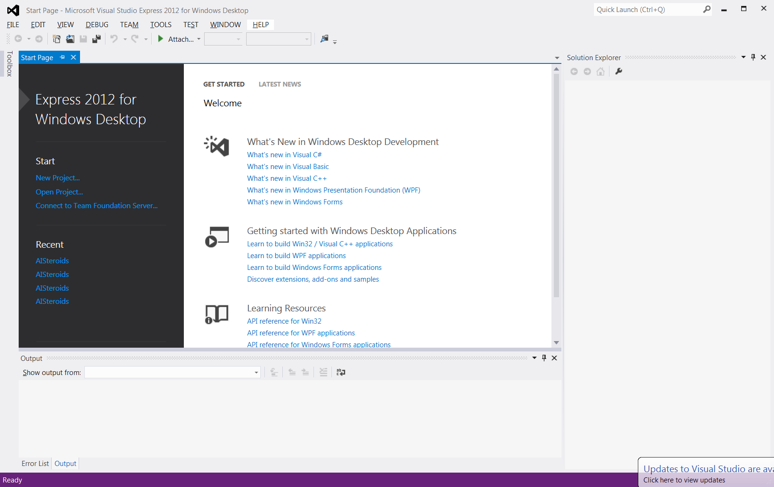
\includegraphics[scale=0.6]{images/vshelp}
			\end{figure}
			\begin{figure}[H]
			\centering
			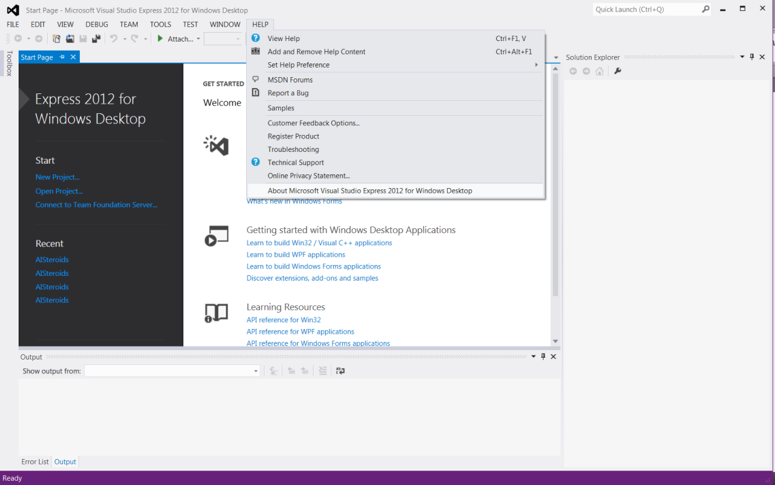
\includegraphics[scale=0.6]{images/vsabout}
		\end{figure}
	\end{itemize}
\end{itemize}
\subsection{CMake}

To check if cmake is installed:\\\\
\texttt{\$ which cmake}\\\\
To check the version number:\\\\
\texttt{\$ cmake --version}\\\\
The minimum required version is 2.8. However, we recommend to use version 3.2 or later. \\

\subsection{CUDA Toolkit}
CUDA is required to compile the GPU executable in both Windows and Linux. However, is not required to compile the CPU code.  To download and install CUDA visit NVIDIA's webpage:\\\\
\url{https://developer.nvidia.com/cuda-downloads}\\
\url{https://developer.nvidia.com/cuda}\\\\

Please refer to CUDA Developer webpages to select an appropriate version for the desired platform. 
To install CUDA in Linux root/sudo, privileges are generally required.  In Windows, administrative access is required.\\\\
To check if nvcc is installed:\\\\
\texttt{\$ which nvcc}\\\\
To check the version number:\\\\
\texttt{\$ nvcc --version}\\\\
The GPU builds of the code requires NVIDIA's CUDA 8.0 or newer:\\\\


%RECOMMENDED SOFTWARE
\section{Recommended Software Tools}
The listed programs are used in this manual and are generally considered necessary.

\subsection{Packmol}
Packmol is a free molecule packing tool (written in Fortran), created by Jos\'e Mario Mart\'inez, a professor of mathematics at the State University of Campinas, Brazil.  Packmol allows a specified number of molecules to be packed at defined separating distances within a certain region of space.  More information regarding downloading and installing Packmol is available on their homepage:\\\\
\url{http://www.ime.unicamp.br/~martinez/packmol}\\\\

\textit{\colorbox{red}{WARNING}}: One of Packmol's limitations is that it is unaware of topology; it treats each molecule or group of molecules as a rigid set of points. It is highly suggested to used the optimized structure of the molecule as the input file to packmol.\\

\textit{\colorbox{red}{WARNING}}: Another more serious limitation is that it is not aware of periodic boundary conditions (PBC).  As a result, when using Packmol to pack PDBs for GOMC, it is recommended to pack to a box 1 Angstroms smaller than the simulation box size.  This prevents hard overlaps over the periodic boundary.\\\\


\subsection{VMD}
VMD (Visual Molecular Dynamics) is a 3-D visualization and manipulation engine for molecular systems written in C-language. VMD is distributed and maintained by the University of Illinois at Urbana-Champaign.  Its sources and binaries are free to download. It comes with a robust scripting engine, which is capable of running python and tcl scripts.
More info can be found here:\\\\
\url{http://www.ks.uiuc.edu/Research/vmd/}\\\\
Although GOMC uses the same fundamental file types ? PDB (coordinates) and PSF (topology) as VMD, it uses some special tricks to obey certain rules of those file formats.\\
One useful purpose of VMD is visualization and analyze your systems.
\begin{figure}[H]
\centering
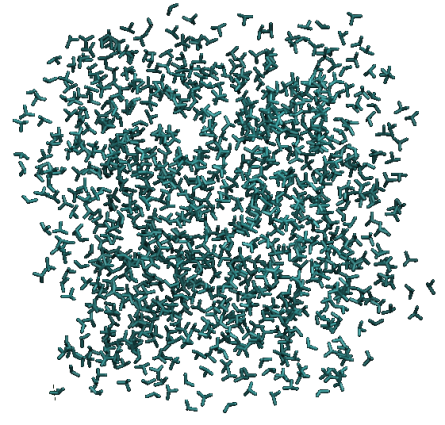
\includegraphics[scale=0.6]{images/vmd}
\caption{A system of united atom isobutane molecules}
\end{figure}
Nonetheless, the most critical part of VMD is a tool called PSFGen.  PSFGen uses a tcl or python script to generate a PDB and PSF file for a system of one or more molecules.  It is, perhaps, the most convenient way to generate a compliant PSF file.
\begin{figure}[H]
\centering
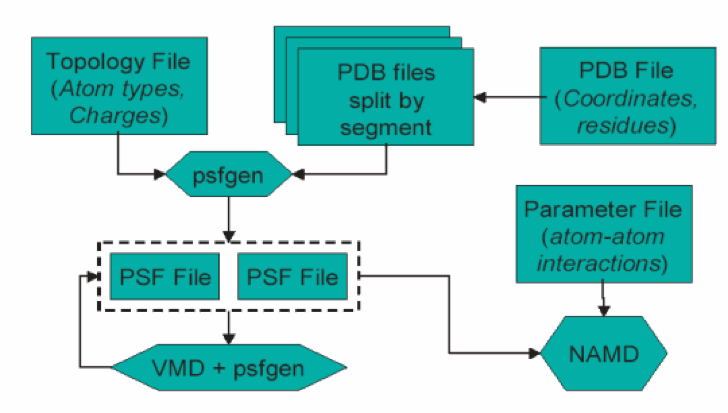
\includegraphics[scale=0.6]{images/psfgen}
\caption{An overview of the PSFGen file generation process and its relationship to VMD/NAMD}
\end{figure}
To read more about PSFGen, reference:\\\\
Plugin homepage @ UIUC\\
\url{http://www.ks.uiuc.edu/Research/vmd/plugins/psfgen}\\\\
``Generating a Protein Structure File (PSF)", part of the NAMD Tutorial from UIUC\\
\url{http://www.ks.uiuc.edu/Training/Tutorials/namd/namd-tutorial-html/node6.html}\\\\
In-Depth Overview [PDF]\\
\url{http://www.ks.uiuc.edu/Research/vmd/plugins/psfgen/ug.pdf}\\\\

%GET SOFTWARE

\section{How to get the software}
The CPU and GPU code are merged together under GOMC project. Currently, version control is handled through the GitHub repository. The latest GOMC release, Example files, and User Manual can be downloaded from GOMC website or GitHub repository.

\subsection{GitHub}
The posted builds in Master branch are ``frozen" versions of the code that have been validated for a number of systems and ensembles. Other branches are created as a means of implementing new features. The latest updated code builds, manual, example files, and other resources can be obtained via the following GitHub repository:\\\\
\url{https://github.com/GOMC-WSU}

\begin{figure}[H]
\centering
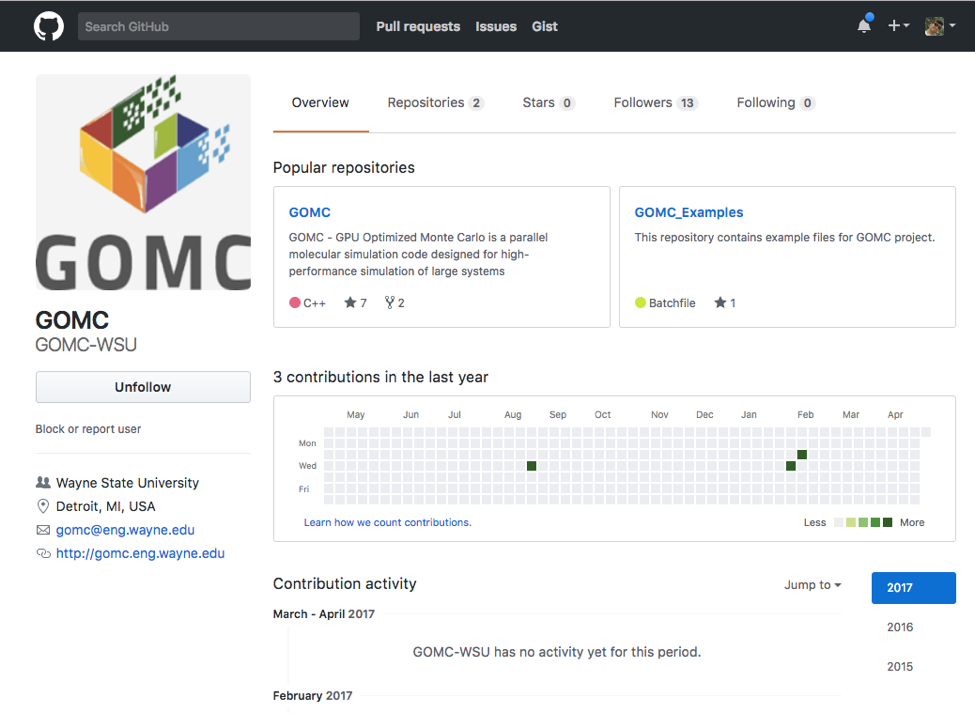
\includegraphics[scale=0.6]{images/github}
\end{figure}

GOMC and Examples repository can be found under the main page. Under GOMC repository, the code and manual can be found. Each repository can be downloaded by clicking on the Clone or download tab. 

\begin{figure}[H]
\centering
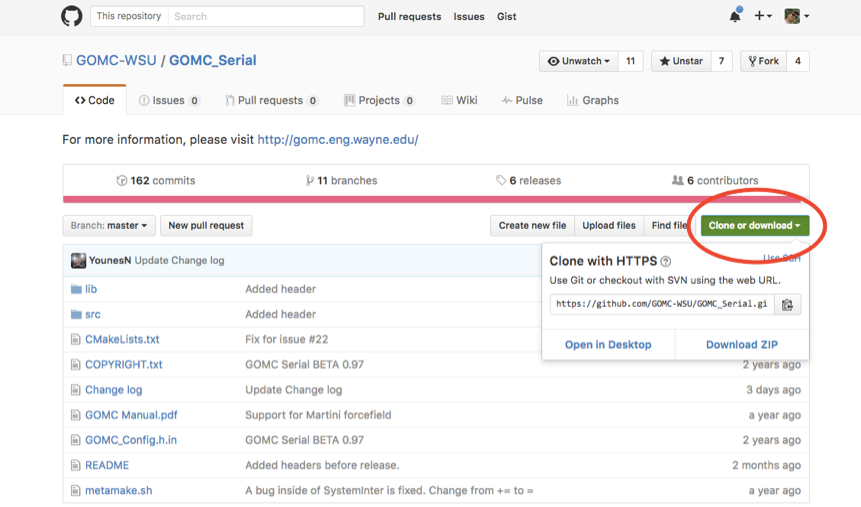
\includegraphics[scale=0.8]{images/clone}
\end{figure}

\subsection{Website}
To access the GOMC website, please click on the following link:\\\\
\url{http://gomc.eng.wayne.edu/} \\\\
The code can be found under the download tab, below and to the right of the logo.  When new betas (or release builds) are announced, they will replace the prior code under the downloads tab.  An announcement will be posted on the front page to notify users.

\begin{figure}[H]
\centering

\includegraphics[scale=0.15]{images/website}
\end{figure}

GOMC is distributed as a compressed folder, containing the source and build system. To compile the code after downloading it, the first step is to extract the compressed build folder.\\
In Linux, the GPU and CPU codes are compressed using gzip and tar (*.tar.gz).  To extract, simply move to the desire folder and type in the command line:\\\\
\texttt{\$ tar -xzvf <file name>.tar.gz}\\\\

%COMLILING
\section{Compiling GOMC}
GOMC generates four executable files for CPU code; \texttt{GOMC\_CPU\_GEMC} (Gibbs ensemble), \texttt{GOMC\_CPU\_NVT} (NVT ensemble), \texttt{GOMC\_CPU\_NPT} (isobaric-isothermal ensemble), and \texttt{GOMC\_CPU\_GCMC} (Grand canonical ensemble). In case of installing CUDA Toolkit, GOMC will generate additional four executable files for GPU code; \texttt{GOMC\_GPU\_GEMC}, \texttt{GOMC\_GPU\_NVT}, \texttt{GOMC\_GPU\_NPT}, and \texttt{GOMC\_GPU\_GCMC}. \\
This section guid users to compile GOMC in Linux or Windows.

\subsection{Linux}
First, navigate your command line to the GOMC base directory. To compile GOMC on Linux, give permission to ``metamake.sh" by running the following command and execute it.\\\\
\texttt{\$ chmod   u+x   metamake.sh}\\
\texttt{\$ ./metamake.sh}\\\\
This script will create a bin directory and run cmake file to compile the code as well. All executable files will be generated in the ``bin" directory.\\

\subsection{Windows}
To compile GOMC on in Windows, follow these steps:
\begin{enumerate}
\item Open the Windows-compatible CMake GUI.
\item Set the Source Folder to the GOMC root folder.
\item Set the build Folder to your Build Folder.
\item Click configure, select your compiler/environment
\item Wait for CMake to finish the configuration.
\item Click configure again and click generate.
\item Open the CMake-generated project/solution etc. to the desired IDE (e.g Visual Studio).
\item Using the solution in the IDE of choice build GOMC per the IDE's standard release compilation/executable generation methods.
\end{enumerate}

\textit{\colorbox{yellow}{NOTE}}: You can also use CMake from the Windows command line if its directory is added to the PATH environment variable.


\subsection{Configuring CMake}
subsubsection{Configure CMAKE}
GOMC use CMAKE to generate multi-platform intermediate files to compile the project. In this section, you can find all the information needed to configure CMAKE.\\
We recommend using a different directory for the cmake output than the home directory of the project as cmake tend to generate lots of files.\\
CMake has a ridiculously expansive set of options, so this document will only reproduce the most obviously relevant ones. When possible, options should be passed into CMake via command line options rather than the CMakeCached.txt file:
\begin{description}
\item [CMAKE\_BUILD\_TYPE] To get the best performance you should build the project in release mode. In cmake GUI you can set the value of ``CMAKE\_BUILD\_TYPE'' to ``Release'' and in cmake command line you can add the following to the cmake:\\\\
\texttt{-DCMAKE\_BUILD\_TYPE=Release}\\\\
To compile the GOMC in debug mode, in cmake GUI, change the value of ``CMAKE\_BUILD\_TYPE'' to ``Debug'' and in cmake command line you can add the following to the cmake:\\\\
\texttt{-DCMAKE\_BUILD\_TYPE=Debug}\\\\
Other options are ``$<$ None $\mid$ ReleaseWithDebInfo $\mid$ MinSizeRel $>$''.
\item [CMAKE\_CXX\_COMPILER] This option will set the compiler. It is recommended to use the Intel Compiler and linking tools, if possible (icc/icpc/etc.). They significantly outperform the default GNU and Visual Studio compiler tools and are available for free for academic use with registration.

\item [CMAKE\_CXX\_FLAGS\_RELEASE:STRING] To run the parallel version of CPU code, it needs to be compiled with openmp library. Open the file ``\texttt{CMakeCache.txt}", while still in the ``bin" folder, and change the value from ``-O3   -DNDEBUG" to ``-O3   -qopenmp   -DNDEBUG". Recompile the GOMC by typing the command:\\\\
\texttt{\$ make}\\

\item [ENSEMBLE\_NVT] You can turn the compilation of CPU version of NVT ensemble on or off using this option.\\
\texttt{-DENSEMBLE\_NVT=$<$On $\mid$ Off $>$}
\item [ENSEMBLE\_NPT] You can turn the compilation of CPU version of NPT ensemble on or off using this option.\\
\texttt{-DENSEMBLE\_NPT=$<$On $\mid$ Off $>$}
\item [ENSEMBLE\_GCMC] You can turn the compilation of CPU version of GCMC ensemble on or off using this option.\\
\texttt{-DENSEMBLE\_GCMC=$<$On $\mid$ Off $>$}
\item [ENSEMBLE\_GEMC] You can turn the compilation of CPU version of GEMC ensemble on or off using this option.\\
\texttt{-DENSEMBLE\_GEMC=$<$On $\mid$ Off $>$}
\item [ENSEMBLE\_GPU\_NVT] You can turn the compilation of GPU version of NVT ensemble on or off using this option.\\
\texttt{-DENSEMBLE\_GPU\_NVT=$<$On $\mid$ Off $>$}
\item [ENSEMBLE\_GPU\_NPT] You can turn the compilation of GPU version of NPT ensemble on or off using this option.\\
\texttt{-DENSEMBLE\_GPU\_NPT=$<$On $\mid$ Off $>$}
\item [ENSEMBLE\_GPU\_GCMC] You can turn the compilation of GPU version of GCMC ensemble on or off using this option.\\
\texttt{-DENSEMBLE\_GPU\_GCMC=$<$On $\mid$ Off $>$}
\item [ENSEMBLE\_GPU\_GEMC] You can turn the compilation of GPU version of GEMC ensemble on or off using this option.\\
\texttt{-DENSEMBLE\_GPU\_GEMC=$<$On $\mid$ Off $>$}
\end{description}

\newpage

%INPUT FILE
\section{Input File Formats}
In order to run simulation in GOMC, the following files need to be provided:
\begin{itemize}
\item GOMC executable
\item PDB file(s)
\item PSF file(s)
\item Parameter file
\item Input file ``NAME.conf" (proprietary control file)\\\\
\end{itemize}

%PDB FILE
\subsection{PDB File}
GOMC requires only one PDB file for NVT and NPT ensembles. However, GOMC requires two PDB files for GEMC and GCMC ensembles.
\subsubsection{What is PDB file}
The term PDB can refer to the Protein Data Bank (\url{http://www.rcsb.org/pdb/}), to a data file provided there, or to any file following the PDB format. Files in the PDB include various information such as the name of the compound, the ATOM and HETATM records containing the coordinates of the molecules, and etc. PDB widely used by NAMD, GROMACS, CHARMM, ACEMD, and Amber. GOMC ignore everything in a PDB file except for the \texttt{REMARK},  \texttt{CRYST1},  \texttt{ATOM}, and  \texttt{END} records. An overview of the PDB standard can be found here:\\\\
\url{http://www.wwpdb.org/documentation/file-format-content/format33/sect2.html#HEADER}\\
\url{http://www.wwpdb.org/documentation/file-format-content/format33/sect8.html#CRYST1}\\
\url{http://www.wwpdb.org/documentation/file-format-content/format33/sect9.html#ATOM}\\

 
PDB contains foure major parts; \texttt{REMARK}, \texttt{CRYST1}, \texttt{ATOM}, and \texttt{END}. Here is the definition of each field and how GOMC is using them to get the information it requires.
\begin{itemize}
\item \texttt{REMARK}: This header records present experimental details, annotations, comments, and information not included in other records (\url{http://www.wwpdb.org/documentation/file-format-content/format33/sect2.html#HEADER}). However, GOMC uses this header to print simulation informations.
	\subitem \textbf{Max Displacement} ($\AA$)
	\subitem \textbf{Max Rotation} (Degree)
	\subitem \textbf{Max volume exchange} ($\AA^3$)
	\subitem \textbf{Monte Carlo Steps} (MC)
\item \texttt{CRYST1}: This header records the unit cell dimension parameters (\url{http://www.wwpdb.org/documentation/file-format-content/format33/sect8.html#CRYST1}).
	\subitem \textbf{Lattice constant: $a, b, c$} ($\AA$)
	\subitem \textbf{Lattice angles: $\alpha , \beta,  \gamma$} (Degree)
\item \texttt{ATOM}: The ATOM records present the atomic coordinates for standard amino acids and nucleotides. They also present the occupancy and temperature factor for each atom (\url{http://www.wwpdb.org/documentation/file-format-content/format33/sect9.html#ATOM}).
	\subitem \textbf{ATOM}: Record name.
	\subitem \textbf{serial}: Atom serial number.
	\subitem \textbf{name}: Atom name.
	\subitem \textbf{resName}: Residue name.
	\subitem \textbf{chainID}: Chain identifier.
	\subitem \textbf{resSeq}: Residue sequence number.
	\subitem \textbf{x}: Coordinates for X ($\AA$).
	\subitem \textbf{y}: Coordinates for Y ($\AA$).
	\subitem \textbf{z}: Coordinates for Z ($\AA$).
	\subitem \textbf{occupancy}: GOMC uses to define which atoms belong to which box.
	\subitem \textbf{beta}: Beta orTemperature factor. GOMC uses this value to define the mobility of the atoms.
	\subitem \textbf{element}: Element symbol.
	\item \texttt{END}: A frame in the PDB file is terminated with the keyword.
\end{itemize} 



Here are the PDB output of GOMC for the first molecule of isobutane:\\

\colorbox{lightgray}{
\begin{tabular}{l *{10}{r}}
  \texttt{REMARK} & \texttt{GOMC} &  \texttt{122.790} &  \texttt{3.14159} &   \texttt{3439.817} &   \texttt{1000000} & & &  & & \\
  \texttt{CRYST1} & \texttt{35.245} & \texttt{35.245} & \texttt{35.245} & \texttt{90.00} & \texttt{90.00} & \texttt{90.00} & & &  & \\
  \texttt{ATOM} & \texttt{1} & \texttt{C1} & \texttt{ISB} & \texttt{1} & \texttt{0.911} & \texttt{-0.313} & \texttt{0.000} & \texttt{0.00} & \texttt{0.00} & \texttt{C} \\
  \texttt{ATOM} & \texttt{2} & \texttt{C2} & \texttt{ISB} & \texttt{1} & \texttt{1.424} & \texttt{-1.765} & \texttt{0.000} & \texttt{0.00} & \texttt{0.00} & \texttt{C} \\
  \texttt{ATOM} & \texttt{3} & \texttt{C3} & \texttt{ISB} & \texttt{1} & \texttt{-0.629} & \texttt{-0.313} & \texttt{0.000} & \texttt{0.00} & \texttt{0.00} & \texttt{C} \\
  \texttt{ATOM} & \texttt{4} & \texttt{C4} & \texttt{ISB} & \texttt{1} & \texttt{1.424} & \texttt{0.413} & \texttt{-1.257} & \texttt{0.00} & \texttt{0.00} & \texttt{C} \\
  \multicolumn{11}{l}{\texttt{END}} \\
\end{tabular} 
} \\\\

The fields seen here in order from left to right are the record type, atom ID, atom name, residue name, residue ID, x, y, and z coordinates, occupancy, temperature factor (called beta), and segment name.\\\\
The atom name is ``C1" and residue name is ``ISB". The PSF file (next section) contains a lookup table of atoms. These contain the atom name from the PDB and the name of the atom kind in the parameter file it corresponds to. As multiple different atom names will all correspond to the same parameter, these can be viewed ``atom aliases" of sorts.  The chain letter (in this case `A') is sometimes used when packing a number of PDBs into a single PDB file.\\

\colorbox{red}{Important}: NOTE on PDB Format Conventions:
\begin{itemize}
\item VMD requires a constant number of ATOMs in a multi-frame PDB (multiple records terminated by ``END" in a single file). To compensate for this, all atoms from all boxes in the system are written to the output PDBs of this code.
\item For atoms not currently in a box, the coordinates are set to $<0.00, 0.00, 0.00>$. The occupancy is commonly just set to ``1.00" and is left unused by many codes. We recycle this legacy parameter by using it to denote, in our output PDBs, the box a particle is in (box 0  occupancy=0.00 ; box 1  occupancy=1.00)
\item{The beta value in GOMC code is used to define the mobility of the molecule. }
	\subitem \textbf{Beta  = 0.00}: molecule can move and transfer within and between boxes.
	\subitem \textbf{Beta = 1.00}: molecule is fixed in its position.
	\subitem \textbf{Beta = 2.00}: molecule can move within the box but cannot be transferred   between boxes.
\end{itemize} 

\subsubsection{Generating PDB file}
With that overview of the format in mind, the following steps describe how a PDB file is typically built.\\
\begin{enumerate}
\item A single molecule PDB is obtained. In this example, the QM software package Gaussian was used to draw the molecule, which was then edited by hand to adhere to the PDB spec properly. The end result is a PDB for a single molecule:\\\\
\colorbox{lightgray}{
\begin{tabular}{l *8r }
  \texttt{REMARK} & \multicolumn{8}{l}{\texttt{1 File created by GaussView 5.0.8}}  \\
  \texttt{ATOM} & \texttt{1} & \texttt{C1} & \texttt{ISB} & \texttt{1} & \texttt{0.911} & \texttt{-0.313} & \texttt{0.000} & \texttt{C} \\
  \texttt{ATOM} & \texttt{2} & \texttt{C2} & \texttt{ISB} & \texttt{1} & \texttt{1.424} & \texttt{-1.765} & \texttt{0.000} & \texttt{C} \\
  \texttt{ATOM} & \texttt{3} & \texttt{C3} & \texttt{ISB} & \texttt{1} & \texttt{-0.629} & \texttt{-0.313} & \texttt{0.000} & \texttt{C} \\
  \texttt{ATOM} & \texttt{4} & \texttt{C4} & \texttt{ISB} & \texttt{1} & \texttt{1.424} & \texttt{0.413} & \texttt{-1.257} & \texttt{C} \\
  \multicolumn{9}{l}{\texttt{END}} \\
\end{tabular}
}
\item Next, packings are calculated to place the simulation in a region of vapor-liquid coexistence. There are a couple of ways to do this in Gibbs ensemble:
\begin{itemize}
\item Pack both boxes to a single middle density, which is an average of the liquid and vapor densities.
\item Same as previous method, but add a modest amount to axis of one box (e.g. 10-30 A).  This technique can be handy in the constant pressure Gibbs ensemble.
\item Pack one box to the predicted liquid density and the other to the vapor density.
\end{itemize}
A good reference for getting the information needed to estimate packing is the NIST Web Book database of pure compounds:\\\\
\url{http://webbook.nist.gov/chemistry/}\\
\item After packing is determined, a basic pack can be performed with a Packmol script.  Here is one example:\\\\
\colorbox{lightgray}{
\begin{tabular}{l}
\texttt{tolerance 3.0}\\
\texttt{filetype pdb}\\
\texttt{output STEP2\_ISB\_packed\_BOX\_0.pdb}\\\\
\texttt{structure isobutane.pdb}\\
\texttt{number 1000}\\
\texttt{inside cube        0.1  0.1  0.1  70.20}\\
\texttt{end structure}
\end{tabular}
}\\\\

Copy the above text into``\texttt{pack\_isobutane.inp}" file, save it and run the script by typing the following line into the terminal:\\\\
\texttt{\$ ./packmol < pack\_isobutane.inp}\\\\
\end{enumerate}

%PSF FILE
\subsection{PSF File}
GOMC requires only one PSF file for NVT and NPT ensembles. However, GOMC requires two PSF files for GEMC and GCMC ensembles.

\subsubsection{What is PSF file}
Protein structure file (PSF), contains all of the molecule-specific information needed to apply a particular force field to a molecular system. The CHARMM force field is divided into a topology file, which is needed to generate the PSF file, and a parameter file, which supplies specific numerical values for the generic CHARMM potential function. The topology file defines the atom types used in the force field; the atom names, types, bonds, and partial charges of each residue type; and any patches necessary to link or otherwise mutate these basic residues. The parameter file provides a mapping between bonded and nonbonded interactions involving the various combinations of atom types found in the topology file and specific spring constants and similar parameters for all of the bond, angle, dihedral, improper, and van der Waals terms in the CHARMM potential function. PSF file widely used by by NAMD, CHARMM, and X-PLOR.\\\\

The PSF file contains six main sections: remarks, atoms, bonds, angles, dihedrals, and impropers (dihedral force terms used to maintain planarity). Each section starts with a specific header described bellow: \\

\begin{itemize}
\item \texttt{NTITLE}: remarks on the file.\\
The following is taken from a PSF file for isobutane: \\\\
\colorbox{lightgray}{
\begin{tabular}{r l l l l l l l l}
\multicolumn{9}{l}{\texttt{PSF}}\\
\texttt{3} & \multicolumn{8}{l}{\texttt{!NTITLE}} \\
\texttt{REMARKS} & \multicolumn{8}{l}{\texttt{original generated structure x-plor psf file}}\\
\texttt{REMARKS} & \multicolumn{8}{l}{\texttt{topology ./Top\_Branched\_Alkanes.inp}}\\
\texttt{REMARKS} & \multicolumn{8}{l}{\texttt{segment ISB \{ first NONE; last NONE; auto angles dihedrals \}}}\\\\
\end{tabular}
}\\

\item \texttt{NATOM}: Defines the atom names, types, and partial charges of each residue type.
	\subitem \texttt{atom ID}
	\subitem \texttt{segment name} 
	\subitem \texttt{residue ID}
	\subitem \texttt{residue name}
	\subitem \texttt{atom name}
	\subitem \texttt{atom type}
	\subitem \texttt{atom charge}
	\subitem \texttt{atom mass} \\
	The following is taken from a PSF file for isobutane: \\\\
	\colorbox{lightgray}{
\begin{tabular}{r l l l l l l l l}
\texttt{4000} & \multicolumn{8}{l}{\texttt{!NATOM}}\\
\texttt{1} & \texttt{ISB} & \texttt{1} & \texttt{ISB} & \texttt{C1} & \texttt{CH1} & \texttt{0.000000} & \texttt{13.0190} & \texttt{0}\\
\texttt{2} & \texttt{ISB} & \texttt{1} & \texttt{ISB} & \texttt{C2} & \texttt{CH3} & \texttt{0.000000} & \texttt{15.0350} & \texttt{0}\\
\texttt{3} & \texttt{ISB} & \texttt{1} & \texttt{ISB} & \texttt{C3} & \texttt{CH3} & \texttt{0.000000} & \texttt{15.0350} & \texttt{0}\\
\texttt{4} & \texttt{ISB} & \texttt{1} & \texttt{ISB} & \texttt{C4} & \texttt{CH3} & \texttt{0.000000} & \texttt{15.0350} & \texttt{0}\\
\texttt{5} & \texttt{ISB} & \texttt{2} & \texttt{ISB} & \texttt{C1} & \texttt{CH1} & \texttt{0.000000} & \texttt{13.0190} & \texttt{0}\\
\texttt{6} & \texttt{ISB} & \texttt{2} & \texttt{ISB} & \texttt{C2} & \texttt{CH3} & \texttt{0.000000} & \texttt{15.0350} & \texttt{0}\\
\texttt{7} & \texttt{ISB} & \texttt{2} & \texttt{ISB} & \texttt{C3} & \texttt{CH3} & \texttt{0.000000} & \texttt{15.0350} & \texttt{0}\\
\texttt{8} & \texttt{ISB} & \texttt{2} & \texttt{ISB} & \texttt{C4} & \texttt{CH3} & \texttt{0.000000} & \texttt{15.0350} & \texttt{0}
\end{tabular}
}\\\\
The fields in the atom section, from left to right are atom ID, segment name, residue ID, residue name, atom name, atom type, charge, mass, and an unused 0. \\
	
\item \texttt{NBOND}: The covalent bond section lists four pairs of atoms per line. \\
The following is taken from a PSF file for isobutane: \\\\
\colorbox{lightgray}{
\begin{tabular}{r l l l l l l l l}
\texttt{3000} & \texttt{!BOND:} & \multicolumn{7}{l}{bonds}\\
\texttt{1} & \texttt{2} & \texttt{1} & \texttt{3} & \texttt{1} & \texttt{4} & \texttt{5} & \multicolumn{2}{l}{\texttt{6}}\\ 
\texttt{5} & \texttt{7} & \texttt{5} & \multicolumn{2}{l}{\texttt{8}}\\ 
\end{tabular}
}\\

\item \texttt{NTHETA}: The angle section lists three triples of atoms per line. \\
The following is taken from a PSF file for isobutane: \\

\colorbox{lightgray}{
\begin{tabular}{r l l l l l l l l}
\texttt{3000} & \texttt{!NTHETA:} & \multicolumn{7}{l}{\texttt{angles}}\\
\texttt{2} & \texttt{1} & \texttt{4} & \texttt{2} & \texttt{1} & \texttt{3} & \texttt{3} & \texttt{1} & \texttt{4}\\
\texttt{6} & \texttt{5} & \texttt{8} & \texttt{6} & \texttt{5} & \texttt{7} & \texttt{7} & \texttt{5} & \texttt{8}\\
\end{tabular}
}\\

\item \texttt{NPHI}: The dihedral sections list two quadruples of atoms per line. 

\item \texttt{NIMPHI}: The improper sections list two quadruples of atoms per line. GOMC currently does not support improper. For the molecules without dihedral or improper, PDF file look like the following:\\\\
\colorbox{lightgray}{
\begin{tabular}{r l l l l l l l l}
\texttt{0} & \multicolumn{8}{l}{\texttt{!NPHI: dihedrals}}\\
&  & &  &  & &  & & \\
\texttt{0} & \multicolumn{8}{l}{\texttt{!NIMPHI: impropers}}\\
\end{tabular}
}\\

\item (other sections such as cross terms) \\
\end{itemize}

\colorbox{red}{Important}: NOTE on PSF Format Conventions:
\begin{itemize}
\item The PSF file format is a highly redundant file format.  It repeats identical topology of thousands of molecules of a common kind in some cases. GOMC follows the same approach as NAMD, allowing this excess information externally and compiling it in the code.
\item Other sections (e.g. cross terms) contain unsupported or legacy parameters and are ignored.
\item Following the restrictions of VMD, the order of the PSF atoms must match the order in the 
.
\item Improper entries are read and stored, but are not currently used.  Support will eventually be added for this.
\end{itemize}

\subsubsection{Generating PSF file}
The PSF file is typically generated using PSFGen. It is convenient to make a script, such as the example below, to do this:\\\\
\colorbox{lightgray}{
\begin{tabular}{l}
\texttt{psfgen << ENDMOL}\\
\texttt{topology ./Top\_branched\_Alaknes.inp}\\
\texttt{segment ISB\{}\\
\texttt{    pdb ./STEP2\_ISB\_packed\_BOX\_0.pdb}\\
\texttt{    first none}\\
\texttt{    last none}\\
\texttt{\}}\\\\
\texttt{coordpdb ./STEP2\_ISB\_packed\_BOX\_0.pdb ISB}\\\\
\texttt{writepsf ./STEP3\_START\_ISB\_sys\_BOX\_0.psf}\\
\texttt{writepdb ./STEP3\_START\_ISB\_sys\_BOX\_0.pdb}\\
\end{tabular}
}\\\\
Typically, one script is run per box to generate a finalized PDB/PSF for that box. The script requires one additional file, the NAMD-style topology file. While GOMC does not directly read or interact with this file, it's typically used to generate the PSF and, hence, is considered one of the integral file types. It will be briefly discussed in the following section.\\\\


%TOPOLOGY
\subsection{Topology File}
A CHARMM forcefield topology file contains all of the information needed to convert a list of residue names into a complete PSF structure file. The topology is a whitespace separated file format, which contains a list of atoms and their corresponding masses, and a list of residue information (charges, composition, and topology). Essentially, it is a non-redundant lookup table equivalent to the PSF file.\\\\
This is followed by a series of residues, which tell PSFGen what atoms are bonded to a given atom. Each residue is comprised of four key elements:
\begin{itemize}
\item A header beginning with the keyword RESI with the residue name and net charge
\item A body with multiple ATOM entries (not to be confused with the PDB-style entries of the same name), which list the partial charge on the particle and what kind of atom each named atom in a specific molecule/residue is.
\item A section of lines starting with the word BOND contains pairs of bonded atoms (typically 3 per line)
\item A closing section with instructions for PSFGen.
\end{itemize}

Here's an example of topology file for isobutane:\\\\
\colorbox{lightgray}{
\begin{tabular}{l}
\texttt{* Custom top file -- branched alkanes}\\
\texttt{*}\\
\texttt{1  1}\\
\texttt{!}\\
\texttt{MASS   1  CH3  15.035 C !}\\
\texttt{MASS   2  CH1  13.019 C !}\\\\
\texttt{AUTOGENERATE ANGLES DIHEDRALS}\\\\
\texttt{RESI ISB ~~ 0.00 ! isobutane - TraPPE}\\
\texttt{GROUP}\\
\texttt{ATOM C1 CH1    0.00 !    C3}\\
\texttt{ATOM C2 CH3    0.00 ! C2-C1}\\
\texttt{ATOM C3 CH3    0.00 !    C4}\\
\texttt{ATOM C4 CH3    0.00 !}\\
\texttt{BOND C1 C2 C1 C3 C1 C4}\\
\texttt{PATCHING FIRS NONE LAST NONE}\\\\
\texttt{END}
\end{tabular}} \\\\\\
Note that the keyword \texttt{END} must be used to terminate this file and keywords related to the auto-generation process must be placed near the top of the file, after the MASS definitions.\\\\
More in-depth information can be found in the following links:\\
\begin{itemize}
\item{Topology Tutorial}: \url{http://www.ks.uiuc.edu/Training/Tutorials/science/topology/topology-tutorial.pdf}
\item{NAMD Tutorial}: Examining the Topology File (\url{http://www.ks.uiuc.edu/Training/Tutorials/science/topology/topology-html/node4.html})
\item{Developing Topology and Parameter Files}: \url{http://www.ks.uiuc.edu/Training/Tutorials/science/force field-tutorial/force field-html/node6.html}
\item{NAMD Tutorial}: Topology Files (\url{http://www.ks.uiuc.edu/Training/Tutorials/namd/namd-tutorial-win-html/node25.html}) \\
\end{itemize}

%PARAMETER FILE
\subsection{Parameter File(s):}
Currently, GOMC uses a single parameter file and the user has the two kinds of parameter file choices:
\begin{itemize}
\item ``\texttt{CHARMM}" (Chemistry at Harvard Molecular Mechanics) compatible parameter file
\item ``\texttt{EXOTIC}" parameter file
\end{itemize}
If the parameter file type is not specified or if the chosen file is missing, an error will result.\\
Both force field file options are whitespace separated files with sections preceded by a tag. When a known tag (representing a molecular interaction in the model) is encountered, reading of that section of the force field begins.  Comments (anything after a * or !) and whitespace are ignored. Reading concludes when the end of the file is reached or another section tag is encountered.\\\\
\underline{CHARMM format parameter file}\\
\texttt{CHARMM} contains a widely used model for describing energies in Monte Carlo and molecular dynamics simulations. It is intended to be compatible with other codes that use such a format, such as \texttt{NAMD}.
For a general overview of the \texttt{CHARMM} force field, see:\\
\url{http://www.charmmtutorial.org/index.php/The_Energy_Function}\\\\
Here's the basic \texttt{CHARMM} contributions that are supported in GOMC:

\begin{align*}
U_{\texttt{bond}}&=\sum_{\texttt{bonds}} K_b(b-b_0)^2 & U_{\texttt{dihedral}}&=\sum_{\texttt{dihedrals}} K_{\phi} [1+\cos(n\phi - \delta)]\\
U_{\texttt{angle}}&=\sum_{\texttt{angles}} K_{\theta}(\theta-\theta_0)^2 & U_{\texttt{LJ}} &=\sum_{\texttt{nonbonded}} \epsilon_{ij}\left[\left(\frac{R_{min_{ij}}}{r_{ij}}\right)^{12}-2\left(\frac{R_{min_{ij}}}{r_{ij}}\right)^6\right]+ \frac{q_i q_j}{\epsilon r_{ij}} \\
\end{align*}

As seen above, the following are recognized, read and used:
\begin{itemize}
\item \texttt{BONDS}
\begin{itemize}
\item Quadratic expression describing bond stretching based on bond length (b) in Angstrom
\item Typically, it is ignored as bonds are rigid for Monte Carlo simulations. To specify that it is to be ignored, put a very large value i.e. ``999999999999" for $K_b$.
\end{itemize}
\colorbox{yellow}{\texttt{NOTE:}} GOMC does not sample bond stretch.
\begin{figure}[H]
\centering
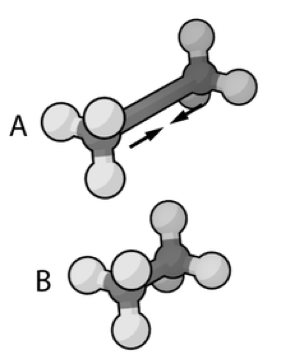
\includegraphics[scale=1.0]{images/bonds}
\caption{Oscillations about the equilibrium bond length}
\end{figure}
\item \texttt{ANGLES}
\begin{itemize}
\item Describe the conformational lbehavior of an angle ($\vartheta$) between three atoms, one of which is shared branch point to the other two. To fix any angle and ignore the related angle energy, put a very large value i.e. ``999999999999" for $K_{\theta}$.
\begin{figure}[H]
\centering
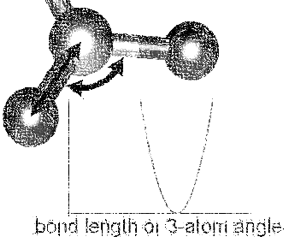
\includegraphics[scale=1.0]{images/angle}
\caption{Oscillations of 3 atoms about an equilibrium bond angle}
\end{figure}
\end{itemize}
\item \texttt{DIHEDRALS} 
\begin{itemize}
\item Describes crankshaft-like rotation behavior about a central bond in a series of three consecutive bonds (rotation is given as $\phi$).
\end{itemize}
\begin{figure}[H]
\centering
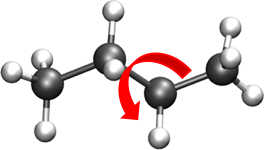
\includegraphics[scale=1.0]{images/dihedrals}
\caption{Torsional rotation of 4 atoms about a central bond}
\end{figure}
\item \texttt{NONBONDED}
\begin{itemize}
\item This tag name only should be used if \texttt{CHARMM} force files are being used. This section describes 12-6 (Lennard-Jones) non-bonded interactions. Non-bonded parameters are assigned by specifying atom type name followed by polarizabilities (which will be ignored), minimum energy, and (minimum radius)/2. In order to modify 1-4 interaction, a second polarizability (again, will be ignored), minimum energy, and (minimum radius)/2 need to be defined; otherwise, the same parameter will be considered for 1-4 interaction.
\end{itemize}
\begin{figure}[H]
\centering
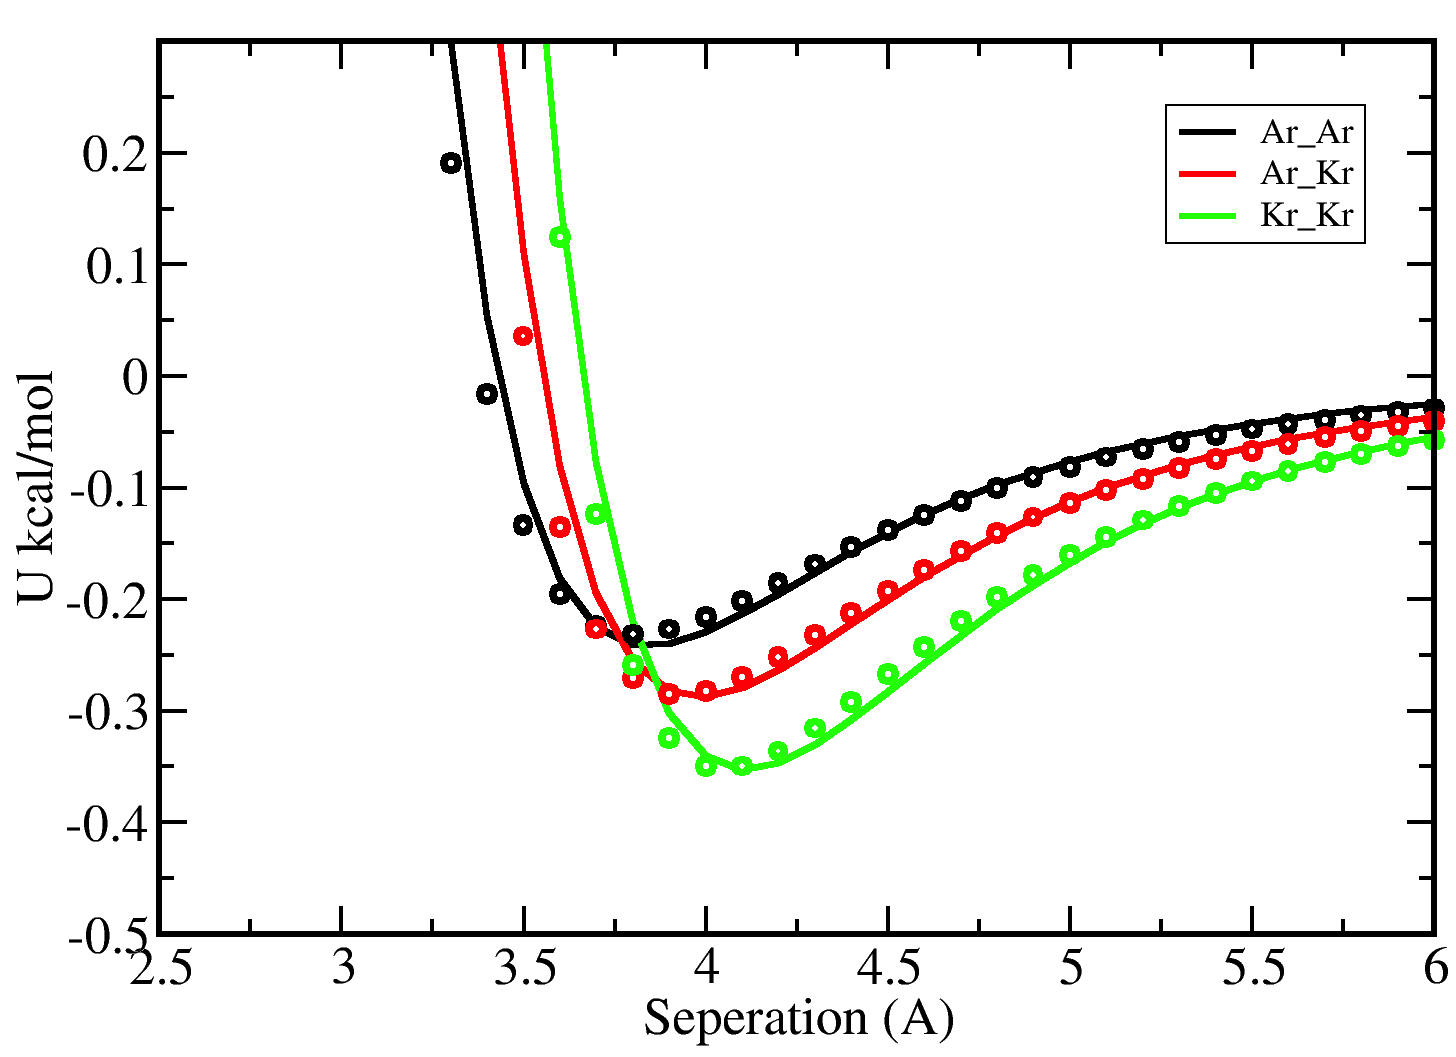
\includegraphics[scale=0.3]{images/nonbonded}
\caption{Non-bonded energy terms (electrostatics and Lenard-Jones)}
\end{figure}

\item \texttt{NBFIX}
\begin{itemize}
\item This tag name only should be used if \texttt{CHARMM} force field is being used. This section allows interaction between two pairs of atoms to be modified, done by specifying two atom type names followed by minimum energy and minimum radius. In order to modify 1-4 interaction, a second minimum energy and minimum radius need to be defined; otherwise, the same parameter will be considered for 1-4 interaction.\\\\
\colorbox{yellow}{\texttt{NOTE:}} Please pay attention that in this section we define minimum radius, not (minimum radius)/2 as it is defined in the \texttt{NONBONDED} section.
\end{itemize}
Currently, supported sections of the \texttt{CHARMM} compliant file include \texttt{BONDS}, \texttt{ANGLES}, \texttt{DIHEDRALS}, \texttt{NONBONDED}, \texttt{NBFIX}. Other sections such as \texttt{CMAP} are not currently read or supported.\\
\end{itemize}
\subsubsection{BONDS}
(``bond stretching") is one key section of the \texttt{CHARMM}-compliant file. Units for the \texttt{$K_b$} variable in this section are in kcal/mol; the \texttt{$b_0$} section (which represents the equilibrium bond length for that kind of pair) is measured in Angstroms.\\\\
\colorbox{lightgray}{
\begin{tabular}{l}
\texttt{BONDS}\\
\texttt{!V(bond) = Kb(b - b0)**2}\\
\texttt{!}\\
\texttt{!Kb: kcal/mole/A**2}\\
\texttt{!b0: A}\\
\texttt{!}\\
\texttt{! Kb (kcal/mol) = Kb (K) * Boltz. const.; }\\
\texttt{!}\\
\texttt{!atom type     Kb              b0        description}\\
\texttt{CH3 CH1        9999999999      1.540   ! TraPPE 2}\\
\end{tabular}}\\\\
\colorbox{yellow}{\texttt{NOTE:}} The \texttt{$K_b$} value may appear odd, but this is because a larger value corresponds to a more rigid bond. As Monte Carlo force fields (e.g. \texttt{TraPPE}) typically treat molecules as rigid constructs, \texttt{$K_b$} is set to a large value - 9999999999. Sampling bond stretch is not supported in GOMC.\\\\
\subsubsection{ANGLES}
(``bond bending"), where \texttt{$\theta$} and \texttt{$\theta_0$} are commonly measured in degrees and \texttt{$K_{\theta}$} is measured in kcal/mol/K.  These values, in literature, are often expressed in Kelvin (K). To convert Kelvin to kcal/mol/K, multiply by the Boltzmann constant -- \texttt{$K_b$} , 0.0019872041 kcal/mol. In order to fix the angle, it requires to set a large value for \texttt{$K_{\theta}$}. By assigning a large value like 9999999999, specified angle will be fixed and energy of that angle will considered to be zero.\\\\
Here is an example of what is necessary for isobutane:\\
\colorbox{lightgray}{
\begin{tabular}{l}
\texttt{ANGLES}\\
\texttt{!}\\
\texttt{!V(angle) = Ktheta(Theta - Theta0)**2}\\
\texttt{!}\\
\texttt{!V(Urey-Bradley) = Kub(S - S0)**2}\\
\texttt{!}\\
\texttt{!Ktheta: kcal/mole/rad**2}\\
\texttt{!Theta0: degrees}\\
\texttt{!S0: A}\\
\texttt{!}\\
\texttt{! Ktheta (kcal/mol) = Ktheta (K) * Boltz. const.}\\
\texttt{!}\\
\texttt{!atom types         Ktheta       Theta0   Kub(?)  S0(?)}\\
\texttt{CH3 CH1 CH3         62.100125    112.00 ! TraPPE 2}\\
\end{tabular}}\\\\
Some CHARMM \texttt{ANGLES} section entries include Urey-Bradley potentials (\texttt{$K_{ub}$}, \texttt{$b_{ub}$}), in addition to the standard quadratic angle potential. The constants related to this potential function are currently read, but the logic has not been added to calculate this potential function. Support for this potential function will be added in later versions of the code.\\
\subsubsection{DIHEDRALS}
The final major bonded interactions section of the \texttt{CHARMM} compliant parameter file are the \texttt{DIHEDRALS}. Each dihedral is composed of a dihedral series of 1 or more terms. Often, there are 4 to 6 terms in a dihedral. Angles for the dihedrals' deltas are given in degrees.\\
Since isobutane has no dihedral, here are the parameters pertaining to 2,3-dimethylbutane:\\\\
\colorbox{lightgray}{
\begin{tabular}{l}
\texttt{DIHEDRALS}\\
\texttt{!}\\
\texttt{!V(dihedral) = Kchi(1 + cos(n(chi) - delta))}\\
\texttt{!}\\
\texttt{!Kchi: kcal/mole}\\
\texttt{!n: multiplicity}\\
\texttt{!delta: degrees}\\
\texttt{!}\\
\texttt{! Kchi (kcal/mol) = Kchi (K) * Boltz. const.}\\
\texttt{!}\\
\texttt{!atom types         Kchi        n    delta              description}\\
\texttt{X   CH1 CH1 X      -0.498907    0       0.0              ! TraPPE 2}\\
\texttt{X   CH1 CH1 X       0.851974    1       0.0              ! TraPPE 2}\\
\texttt{X   CH1 CH1 X      -0.222269    2   180.0              ! TraPPE 2}\\
\texttt{X   CH1 CH1 X       0.876894    3       0.0              ! TraPPE 2}\\
\end{tabular}}\\\\
\colorbox{yellow}{\texttt{NOTE:}} The code allows the use of `X' to indicate ambiguous positions on the ends. This is useful because this kind is often determined solely by the two middle atoms in the middle of the dihedral, according to literature.
\subsubsection{IMPROPERS}
Energy parameters used to describe out-of-plane rocking are currently read, but unused. The section is often blank. If it becomes necessary, algorithms to calculate the improper energy will need to be added.\\

\subsubsection{NONBONDED}
The next section of the \texttt{CHARMM} style parameter file is the \texttt{NONBONDED}. In order to use \texttt{TraPPE} this section of the \texttt{CHARMM} compliant file is critical. Here's an example with our isobutane potential model:\\\\
\colorbox{lightgray}{
\begin{tabular}{l}
\texttt{NONBONDED }\\
\texttt{!}\\
\texttt{!V(Lennard-Jones) = Eps,i,j[(Rmin,i,j/ri,j)**12 - 2(Rmin,i,j/ri,j)**6]}\\
\texttt{!}\\
\texttt{!atom  ignored   epsilon     Rmin/2       ignored  eps,1-4  Rmin/2,1-4}\\
\texttt{!}\\
\texttt{CH3    0.0      -0.194745992  2.10461634058 0.0   0.0   0.0 ! TraPPE 1}\\
\texttt{CH1    0.0      -0.019872040  2.62656119304 0.0   0.0   0.0! TraPPE 2}\\
\texttt{End}\\
\end{tabular}}\\\\
\colorbox{yellow}{\texttt{NOTE:}} The \texttt{$R_{min}$} is different from \texttt{$\sigma$}. \texttt{$\sigma$} is the distance to the x-intercept (where interaction energy goes from being repulsive to positive). \texttt{$R_{min}$} is the potential well-depth, where the attraction is maximum. To convert \texttt{$\sigma$} to \texttt{$R_{min}$}, simply multiply \texttt{$\sigma$} by 0.56123102415, and flag it with a negative sign.\\

\subsubsection{NBFIX}
The last section of the \texttt{CHARMM} style parameter file is the \texttt{NBFIX}. In this section, individual pair interaction will be modified. First, pseudo non-bonded parameters have to be defined in \texttt{NONBONDED} and modified in \texttt{NBFIX}. Here?s an example if it is required to modify interaction between \texttt{CH3} and \texttt{CH1} atoms:\\\\
\colorbox{lightgray}{
\begin{tabular}{l}
\texttt{NBFIX }\\
\texttt{!V(Lennard-Jones) = Eps,i,j[(Rmin,i,j/ri,j)**12 - 2(Rmin,i,j/ri,j)**6]}\\
\texttt{!}\\
\texttt{!atom  atom  epsilon      Rmin  eps,1-4  Rmin,1-4}\\
\texttt{CH3   CH1    -0.294745992 1.10461634058 ! }\\
\texttt{End}\\
\end{tabular}}\\\\

\newpage
\subsection{Exotic Parameter file}
The exotic file is intended for use with nonstandard/specialty models of molecular interaction, which are not included in \texttt{CHARMM} standard. Currently, two custom interaction are included:
\begin{description}
\item [NONBODED\_MIE] This section describes n-6 (Lennard-Jones) non-bonded interactions. The Lennard-Jones potential (12-6) is a subset of this potential. Non-bonded parameters are assigned by specifying atom type name followed by minimum energy, atom diameter, and repulsion exponent. In order to modify 1-4 interaction, a second minimum energy, atom diameter, and repulsion exponent need to be defined; otherwise, the same parameters would be considered for 1-4 interaction.
\item [NBFIX\_MIE] This section allows n-6 (Lennard-Jones) interaction between two pairs of atoms to be modified. This is done by specifying two atoms type names followed by minimum energy, atom diameter, and repulsion exponent. In order to modify 1-4 interaction, a second minimum energy, atom diameter, and repulsion exponent need to be defined; otherwise, the same parameter will be considered for 1-4 interaction.
\end{description}
\colorbox{yellow}{\texttt{NOTE:}} In \texttt{EXOTIC} force field, the definition of atom diameter($\sigma$) is same for both \texttt{NONBONDED\_MIE} and \texttt{NBFIX\_MIE}.\\
Otherwise, the exotic file reuses the same geometry section headings - \texttt{BONDS} / \texttt{ANGLES} / \texttt{DIHEDRALS} / etc. The only difference in these sections versus in the \texttt{CHARMM} format force field file is that the energies are in Kelvin (`K'), the unit most commonly found for parameters in Monte Carlo chemical simulation literature. This precludes the need to convert to kcal/mol, the energy unit used in \texttt{CHARMM}.\\ The most frequently used section of the exotic files in the Mie potential section is \texttt{NONBONDED\_MIE}.\\
Here are the parameters that are used to simulate alkanes:\\\\
\colorbox{lightgray}{
\begin{tabular}{l}
\texttt{NONBONDED\_MIE}\\
\texttt{!}\\
\texttt{!V(mie) = 4*eps*((sig\_ij/r\_ij)\^n-(sig\_ij/r\_ij)\^6)}\\
\texttt{!}\\
\texttt{!atom   eps          sig        n    eps,1-4    sig,1-4     n,1-4 }\\
\texttt{CH4     161.00       3.740      14   0.0 0.0 0.0 ! Potoff, et al. '09}\\
\texttt{CH3     121.25       3.783      16   0.0 0.0 0.0 ! Potoff, et al. '09}\\
\texttt{CH2       61.00       3.990      16   0.0 0.0 0.0 ! Potoff, et al. '09}\\
\end{tabular}}\\\\
\colorbox{yellow}{\texttt{NOTE:}} Although the units (Angstroms) are the same, the exotic file uses $\sigma$, not the $R_{min}$ used by \texttt{CHARMM}. The energy in the exotic file are expressed in Kelvin (K), as this is the standard convention in the literature.\\
\newpage
\subsection{Control File (*.conf)}
The control file is GOMC's proprietary input file. It contains key settings. The settings generally fall under three categories:
\begin{itemize}
\item Input/Simulation Setup
\item System Settings for During Run
\item Output Settings
\end{itemize}
\colorbox{yellow}{\texttt{NOTE:}} The control file is designed to recognize logic values, such as ``yes/true/on" or ``no/false/off".\\
\subsubsection{Input/Simulation Setup}
In this section, input file names are listed. In addition, if you want to restart your simulation or use integer seed for running your simulation, you need to modify this section according to your purpose.
\begin{description}
\item [Restart] Determines whether to restart the simulation from previous simulation or not.\\
	\begin{itemize}
	\item Value 1: $<BOOLEAN>$ - true if restart, false otherwise\\
	\end{itemize}
\item [PRNG] Dictates how to start the pseudo-random number generator (PRNG)
	\begin{itemize}
	\item Value 1: $<STRING>$
		\begin{itemize}
		\item \texttt{RANDOM}: Randomizes Mersenne Twister PRNG with random bits based on the system time.
		\colorbox{lightgray}{
		\begin{tabular}{l}
		\texttt{\#\#\#\#\#\#\#\#\#\#\#\#\#\#\#\#\#\#\#\#\#\#\#\#\#\#\#\#\#\#\#\#\#}\\
		\texttt{\# kind \{RANDOM, INTSEED\}}\\
		\texttt{\#\#\#\#\#\#\#\#\#\#\#\#\#\#\#\#\#\#\#\#\#\#\#\#\#\#\#\#\#\#\#\#\#}\\
		\texttt{PRNG RANDOM}\\
		\end{tabular}}
		\item \texttt{INTSEED}: This option ``seeds" the Mersenne Twister PRNG with a standard integer. When the same integer is used, the generated PRNG stream should be the same every time, which is helpful in tracking down bugs.\\
		\colorbox{lightgray}{
		\begin{tabular}{l}
		\texttt{\#\#\#\#\#\#\#\#\#\#\#\#\#\#\#\#\#\#\#\#\#\#\#\#\#\#\#\#\#\#\#\#\#}\\
		\texttt{\# kind \{RANDOM, INTSEED\}}\\
		\texttt{\#\#\#\#\#\#\#\#\#\#\#\#\#\#\#\#\#\#\#\#\#\#\#\#\#\#\#\#\#\#\#\#\#}\\
		\texttt{PRNG INTSEED}\\
		\end{tabular}}
		\end{itemize}
	\end{itemize}
\item [Random\_Seed] Defines the seed number. If ``INTSEED" is chosen, seed number needs to be specified; otherwise, the program will terminate.
	\begin{itemize}
	\item Value 1: $<ULONG>$ or $<UINT>$: If ``INTSEED" command is used (See above example).\\
	\colorbox{lightgray}{
	\begin{tabular}{l}
	\texttt{\#\#\#\#\#\#\#\#\#\#\#\#\#\#\#\#\#\#\#\#\#\#\#\#\#\#\#\#\#\#\#\#\#}\\
	\texttt{\# kind \{RANDOM, INTSEED\}}\\
	\texttt{\#\#\#\#\#\#\#\#\#\#\#\#\#\#\#\#\#\#\#\#\#\#\#\#\#\#\#\#\#\#\#\#\#}\\
	\texttt{PRNG INTSEED}\\
	\texttt{Random\_Seed 50}\\
	\end{tabular}}
	\end{itemize}
\item [ParaTypeCHARMM] Sets force field type to \texttt{CHARMM} style.
	\begin{itemize}
	\item Value 1: $<BOOLEAN>$ - true if it is \texttt{CHARMM} force field, false if it is not.\\
	\colorbox{lightgray}{
	\begin{tabular}{l}
	\texttt{\#\#\#\#\#\#\#\#\#\#\#\#\#\#\#\#\#\#\#\#\#\#\#\#\#\#\#\#\#\#\#\#\#}\\
	\texttt{\# FORCE FIELD TYPE}\\
	\texttt{\#\#\#\#\#\#\#\#\#\#\#\#\#\#\#\#\#\#\#\#\#\#\#\#\#\#\#\#\#\#\#\#\#}\\
	\texttt{ParaTypeCHARMM true}\\
	\end{tabular}}
	\end{itemize}
\item [ParaTypeEXOTIC] Sets force field type to \texttt{EXOTIC} style.
	\begin{itemize}	
	\item Value 1: $<BOOLEAN>$ - true if it is \texttt{EXOTIC} force field, false if it is not.\\
	\colorbox{lightgray}{
	\begin{tabular}{l}
	\texttt{\#\#\#\#\#\#\#\#\#\#\#\#\#\#\#\#\#\#\#\#\#\#\#\#\#\#\#\#\#\#\#\#\#}\\
	\texttt{\# FORCE FIELD TYPE}\\
	\texttt{\#\#\#\#\#\#\#\#\#\#\#\#\#\#\#\#\#\#\#\#\#\#\#\#\#\#\#\#\#\#\#\#\#}\\
	\texttt{ParaTypeEXOTIC true}\\
	\end{tabular}}
	\end{itemize}
\item [ParaTypeMARTINI] Sets force field type to MARTINI style.
	\begin{itemize}	
	\item Value 1: $<BOOLEAN>$ - true if it is \texttt{MARTINI} force field, false if it is not.\\
	\colorbox{lightgray}{
	\begin{tabular}{l}
	\texttt{\#\#\#\#\#\#\#\#\#\#\#\#\#\#\#\#\#\#\#\#\#\#\#\#\#\#\#\#\#\#\#\#\#}\\
	\texttt{\# FORCE FIELD TYPE}\\
	\texttt{\#\#\#\#\#\#\#\#\#\#\#\#\#\#\#\#\#\#\#\#\#\#\#\#\#\#\#\#\#\#\#\#\#}\\
	\texttt{ParaTypeMARTINI true}\\
	\end{tabular}}
	\end{itemize}
\item [Parameters] Provides the name and location of the parameter file to use for the simulation.
	\begin{itemize}	
	\item Value 1: $<STRING>$ - Sets the name of the parameter file.\\
	\colorbox{lightgray}{
	\begin{tabular}{l}
	\texttt{\#\#\#\#\#\#\#\#\#\#\#\#\#\#\#\#\#\#\#\#\#\#\#\#\#\#\#\#\#\#\#\#\#}\\
	\texttt{\# FORCE FIELD TYPE}\\
	\texttt{\#\#\#\#\#\#\#\#\#\#\#\#\#\#\#\#\#\#\#\#\#\#\#\#\#\#\#\#\#\#\#\#\#}\\
	\texttt{ParaTypeCHARMM yes}\\
	\texttt{Parameters ../../common/Par\_TraPPE\_Alkanes.inp}\\
	\end{tabular}}
	\end{itemize}
\item [Coordinates] Defines the PDB filenames (coordinates) for each box in the system.
	\begin{itemize}	
	\item Value 1: $<INTEGER>$ - Sets box number (first box is box `0').\\
	\item Value 2: $<STRING>$ - Sets PDB file name\\\\
	\colorbox{yellow}{\texttt{NOTE:}} NVT and NPT ensembles requires only one PDB file and GEMC/GCMC requires two PDB files. If the number of PDB files is not compatible with the simulation type, the program will terminate. \\\\
	Example of NVT or NPT ensemble\\
	\colorbox{lightgray}{
	\begin{tabular}{l}
	\texttt{\#\#\#\#\#\#\#\#\#\#\#\#\#\#\#\#\#\#\#\#\#\#\#\#\#\#\#\#\#\#\#\#\#}\\
	\texttt{\# INPUT PDB FILES - NVT or NPT ensemble}\\
	\texttt{\#\#\#\#\#\#\#\#\#\#\#\#\#\#\#\#\#\#\#\#\#\#\#\#\#\#\#\#\#\#\#\#\#}\\
	\texttt{Coordinates 0 STEP3\_START\_ISB\_sys.pdb}\\
	\end{tabular}}\\\\
	Example of Gibbs or GC ensemble\\
	\colorbox{lightgray}{
	\begin{tabular}{l}
	\texttt{\#\#\#\#\#\#\#\#\#\#\#\#\#\#\#\#\#\#\#\#\#\#\#\#\#\#\#\#\#\#\#\#\#}\\
	\texttt{\# INPUT PDB FILES - Gibbs or GC ensemble}\\
	\texttt{\#\#\#\#\#\#\#\#\#\#\#\#\#\#\#\#\#\#\#\#\#\#\#\#\#\#\#\#\#\#\#\#\#}\\
	\texttt{Coordinates 0 STEP3\_START\_ISB\_sys\_BOX\_0.pdb}\\
	\texttt{Coordinates 1 STEP3\_START\_ISB\_sys\_BOX\_1.pdb}\\
	\end{tabular}}
	
	\colorbox{yellow}{\texttt{NOTE:}} In case of \texttt{Restart   true}, the restart PDB output file from GOMC (OutputName\_BOX\_0\_restart.pdb) can be used for each boxe. \\\\
	Example of Gibbs ensemble when \texttt{Restart} mode is active\\
	\colorbox{lightgray}{
	\begin{tabular}{l}
	\texttt{\#\#\#\#\#\#\#\#\#\#\#\#\#\#\#\#\#\#\#\#\#\#\#\#\#\#\#\#\#\#\#\#\#}\\
	\texttt{\# INPUT PDB FILES}\\
	\texttt{\#\#\#\#\#\#\#\#\#\#\#\#\#\#\#\#\#\#\#\#\#\#\#\#\#\#\#\#\#\#\#\#\#}\\
	\texttt{Coordinates 0 ISB\_T\_270\_k\_BOX\_0\_restart.pdb}\\
	\texttt{Coordinates 1 ISB\_T\_270\_k\_BOX\_1\_restart.pdb}\\
	\end{tabular}}
	\end{itemize}
	
\item [Structures] Defines the PSF filenames (structures) for each box in the system.
	\begin{itemize}	
	\item Value 1: $<INTEGER>$ - Sets box number (first box is box `0').\\
	\item Value 2: $<STRING>$ - Sets PSF file name\\\\
	\colorbox{yellow}{\texttt{NOTE:}} NVT and NPT ensembles requires only one PSF file and GEMC/GCMC requires two PSF files. If the number of PSF files is not compatible with the simulation type, the program will terminate. \\
	
	Example of NVT or NPT ensemble\\
	\colorbox{lightgray}{
	\begin{tabular}{l}
	\texttt{\#\#\#\#\#\#\#\#\#\#\#\#\#\#\#\#\#\#\#\#\#\#\#\#\#\#\#\#\#\#\#\#\#}\\
	\texttt{\# INPUT PSF FILES}\\
	\texttt{\#\#\#\#\#\#\#\#\#\#\#\#\#\#\#\#\#\#\#\#\#\#\#\#\#\#\#\#\#\#\#\#\#}\\
	\texttt{Structure 0 STEP3\_START\_ISB\_sys.psf}\\
	\end{tabular}}\\\\
	Example of Gibbs or GC ensemble\\
	\colorbox{lightgray}{
	\begin{tabular}{l}
	\texttt{\#\#\#\#\#\#\#\#\#\#\#\#\#\#\#\#\#\#\#\#\#\#\#\#\#\#\#\#\#\#\#\#\#}\\
	\texttt{\# INPUT PSF FILES}\\
	\texttt{\#\#\#\#\#\#\#\#\#\#\#\#\#\#\#\#\#\#\#\#\#\#\#\#\#\#\#\#\#\#\#\#\#}\\
	\texttt{Structure 0 STEP3\_START\_ISB\_sys\_BOX\_0.psf}\\
	\texttt{Structure 1 STEP3\_START\_ISB\_sys\_BOX\_1.psf}\\
	\end{tabular}}
	
	\colorbox{yellow}{\texttt{NOTE:}} In case of \texttt{Restart   true}, the PSF output file from GOMC (OutputName\_merged.psf) can be used for both boxes. \\\\
	Example of Gibbs ensemble when Restart mode is active\\
	\colorbox{lightgray}{
	\begin{tabular}{l}
	\texttt{\#\#\#\#\#\#\#\#\#\#\#\#\#\#\#\#\#\#\#\#\#\#\#\#\#\#\#\#\#\#\#\#\#}\\
	\texttt{\# INPUT PSF FILES}\\
	\texttt{\#\#\#\#\#\#\#\#\#\#\#\#\#\#\#\#\#\#\#\#\#\#\#\#\#\#\#\#\#\#\#\#\#}\\
	\texttt{Structure 0 ISB\_T\_270\_k\_merged.psf}\\
	\texttt{Structure 1 ISB\_T\_270\_k\_merged.psf}\\
	\end{tabular}}
	\end{itemize}
	
\end{description}

\subsubsection{System Settings for During Run Setup}
This section contains all the variables not involved in the output of data during the simulation, or in the reading of input files at the start of the simulation.  In other words, it contains settings related to the moves, the thermodynamic constants (based on choice of ensemble), and the length of the simulation.\\
Note that some tags, or entries for tags, are only used in certain ensembles (e.g. Gibbs ensemble). These cases are denoted with colored text.\\
\begin{description}
\item [GEMC] \colorbox{cyan}{(For Gibbs Ensemble runs only)} Defines what type of Gibbs Ensemble simulation you want to run.\\
	If neglected in Gibbs Ensemble, it simply defaults to constant volume (NVT) Gibbs Ensemble.
	\begin{itemize}
	\item Value 1: $<STRING>$ - allows you to pick between isovolumetric (``NVT") and isobaric (``NPT") Gibbs ensemble simulations
		\begin{itemize}
		\item NVT: Run simulation with constant molecule number, volume, and temperature.\\
		\item NPT: Run simulation with constant molecule number, pressure, and temperature.\\
		\colorbox{lightgray}{
		\begin{tabular}{l}
		\texttt{\#\#\#\#\#\#\#\#\#\#\#\#\#\#\#\#\#\#\#\#\#\#\#\#\#\#\#\#\#\#\#\#\#}\\
		\texttt{\# GEMC TYPE (DEFAULT IS NVT\_GEMC}\\
		\texttt{\#\#\#\#\#\#\#\#\#\#\#\#\#\#\#\#\#\#\#\#\#\#\#\#\#\#\#\#\#\#\#\#\#}\\
		\texttt{GEMC    NVT}\\
		\end{tabular}}
		\end{itemize}
	\end{itemize}
\item [Pressure] If ``NPT" simulation is chosen, imposed pressure (in bar) needs to be specified; otherwise, the program will terminate.
	\begin{itemize}
	\item Value 1: $<DOUBLE>$ - Constant pressure in bars.\\
	\colorbox{lightgray}{
	\begin{tabular}{l}
	\texttt{\#\#\#\#\#\#\#\#\#\#\#\#\#\#\#\#\#\#\#\#\#\#\#\#\#\#\#\#\#\#\#\#\#}\\
	\texttt{\# GEMC TYPE (DEFAULT IS NVT\_GEMC}\\
	\texttt{\#\#\#\#\#\#\#\#\#\#\#\#\#\#\#\#\#\#\#\#\#\#\#\#\#\#\#\#\#\#\#\#\#}\\
	\texttt{GEMC    NPT}\\
	\texttt{Pressure 5.76}\\
	\end{tabular}}
	\end{itemize}
\item [Temperature] Sets the temperature at which the system will run.
	\begin{itemize}
	\item Value 1: $<DOUBLE>$ - Constant temperature of simulation in degrees Kelvin.
	\end{itemize}
\item [Rcut] Sets a specific radius that non-bonded interaction energy and force will be considered and calculated using defined potential function.
	\begin{itemize}
	\item Value 1: $<DOUBLE>$ - The distance to truncate the Lennard-Jones potential at.
	\end{itemize}	
\item [RcutLow] Sets a specific minimum possible in angstrom that reject any move that place any atom closer than specified distance.
	\begin{itemize}
	\item Value 1: $<DOUBLE>$ - The minimum possible distance between any atoms.
	\end{itemize}
\item [LRC] Defines whether or not long range corrections are used.
	\begin{itemize}
	\item Value 1: $<BOOLEAN>$ - True to consider long range correction. In case of using ``SHIFT" or ``SWITCH" potential functions, LRC will be ignored.
	\end{itemize}
\item [Exclude] Defines which pairs of bonded atoms should be excluded from non-bonded interactions.
	\begin{itemize}
	\item Value 1: $<STRING>$ - Allows you to choose between ``1-2", ``1-3", and ``1-4".
		\begin{description}
		\item [1-2] All interactions pairs of bonded atoms, except the ones that separated with one bond, will be considered and modified using 1-4 parameters defined in parameter file.
		\item [1-3] All interaction pairs of bonded atoms, except the ones that separated with one or two bonds, will be considered and modified using 1-4 parameters defined in parameter file.
		\item [1-4] All interaction pairs of bonded atoms, except the ones that separated with one, two or three bonds, will be considered using non-bonded parameters defined in parameter file.
		\end{description}
		\colorbox{yellow}{\texttt{NOTE:}} The default value is ``1-4".\\
		\colorbox{yellow}{\texttt{NOTE:}} In CHARMM force field, the 1-4 interaction needs to be considered. Choosing ``Exclude 1-3'' will modify 1-4 interaction based on 1-4 parameter in parameter file. If a kind force field is used, where 1-4 interaction needs to be ignored, such as TraPPE, either ``exclude 1-4'' needs to be chosen or 1-4 parameter needs to be assigned a value of zero in the parameter file.
	\end{itemize}
\item [Potential] Defines the potential function type to calculate non-bonded interaction energy and force between atoms.
	\begin{itemize}
	\item Value 1: $<STRING>$ - Allows you to pick between ``VDW'', ``SHIFT'' and ``SWITCH''.
		\begin{description}
		\item [VDW] Nonbonded interaction energy and force calculated based on n-6 (Lennard-Johns) equation. This function will be discussed further in the Intermolecular energy and Virial calculation section.\\
		\colorbox{lightgray}{
		\begin{tabular}{l}
		\texttt{\#\#\#\#\#\#\#\#\#\#\#\#\#\#\#\#\#\#\#\#\#\#\#\#\#\#\#\#\#\#\#\#\#}\\
		\texttt{\# SIMULATION CONDITION}\\
		\texttt{\#\#\#\#\#\#\#\#\#\#\#\#\#\#\#\#\#\#\#\#\#\#\#\#\#\#\#\#\#\#\#\#\#}\\
		\texttt{Temperature 270.00}\\
		\texttt{Potential VDW}\\
		\texttt{LRC true}\\
		\texttt{Rcut 10}\\
		\texttt{Exclude 1-4}\\
		\end{tabular}}
		\item [SHIFT] This option forces the potential energy to be zero at Rcut distance. This function will be discussed further in the Intermolecular energy and Virial calculation section.\\
		\colorbox{lightgray}{
		\begin{tabular}{l}
		\texttt{\#\#\#\#\#\#\#\#\#\#\#\#\#\#\#\#\#\#\#\#\#\#\#\#\#\#\#\#\#\#\#\#\#}\\
		\texttt{\# SIMULATION CONDITION}\\
		\texttt{\#\#\#\#\#\#\#\#\#\#\#\#\#\#\#\#\#\#\#\#\#\#\#\#\#\#\#\#\#\#\#\#\#}\\
		\texttt{Temperature 270.00}\\
		\texttt{Potential SHIFT}\\
		\texttt{LRC false}\\
		\texttt{Rcut 10}\\
		\texttt{Exclude 1-4}\\
		\end{tabular}}
		\item [SWITCH] This option smoothly forces the potential energy to be zero at $R_{cut}$ distance and starts modifying the potential at \texttt{Rswitch} distance. Depending on force field type, specific potential function will be applied. These functions will be discussed further in the Intermolecular energy and Virial calculation section.
		\end{description}
	\end{itemize}
\item [Rswitch] In the case of choosing “SWITCH” as potential function, a distance is set in which non-bonded interaction energy is truncated smoothly from to cutoff distance.
	\begin{itemize}
	\item Value 1: $<DOUBLE>$ - Define switch distance in angstrom. If the ``SWITCH'' function is chosen, \texttt{Rswitch} needs to be defined; otherwise, the program will be terminated. 
	\end{itemize}
\item [ElectroStatic] Considers coulomb interaction or not. This function will be discussed further in the Intermolecular energy and Virial calculation section.
	\begin{itemize}
	\item Value 1: $<BOOLEAN>$ - True if coulomb interaction needs to be considered and false if not.
	\end{itemize}
	\colorbox{yellow}{\texttt{NOTE:}} If MARTINI force field was used and charged molecule was used in simulation, ElectroStatic needs to be turn on. MARTINI force field uses short range coulomb interaction with constant dielectric 15.0.
\item [Ewald] Considers standard Ewald summation method for electrostatic calculation. This function will be discussed further in the Intermolecular energy and Virial calculation section.
	\begin{itemize}
	\item Value 1: $<DOUBLE>$ - ``true'' if Ewald summation calculation needs to be considered and ``false'' if not.
	\end{itemize}
	\colorbox{yellow}{\texttt{NOTE:}} By default, \texttt{ElectroStatic} will be set to true if Ewald summation method was used to calculate coulomb interaction.
\item [CachedFourier] Considers storing the reciprocal terms for Ewald summation calculation in order to improve the code performance. This option would increase the code performance with the cost of memory usage.
	\begin{itemize}
	\item Value 1: $<BOOLEAN>$ - ``true'' to store reciprocal terms of Ewald summation calculation and ``false'' if not.
	\end{itemize}
	\colorbox{yellow}{\texttt{NOTE:}} By default, \texttt{CachedFourier} will be set to ``true'' if not value was set.
\item [Tolerance] Specifies the accuracy of the Ewald summation calculation. Ewald separation parameter and number of reciprocal vectors for the Ewald summation are determined based on the accuracy parameter.
	\begin{itemize}
	\item Value 1: $<DOUBLE>$ - Sets the accuracy in Ewald summation calculation. A reasonable value for te accuracy is 0.00001.
	\end{itemize}
	\colorbox{yellow}{\texttt{NOTE:}} If ``Ewald'' was chosen and no value was set for Tolerance, the program will be terminated.
\item [Dielectric] Defines dielectric constant for coulomb interaction in MARTINI force field.
	\begin{itemize}
	\item Value 1: $<DOUBLE>$ - Sets dielectric value used in coulomb interaction.
	\end{itemize}
	\colorbox{yellow}{\texttt{NOTE:}} In MARTINI force field, \texttt{Dielectric} needs to be set to 15.0. If MARTINI force field was chosen and if \texttt{Dielectric} was not specified, a default value of 15.0 will be assigned.
\item [PressureCalc] Considers to calculate the pressure or not. If it is set to true, the frequency of pressure calculation need to be set.
	\begin{itemize}
	\item Value 1: $<BOOLEAN>$ - ``True'' enabling pressure calculation during the simulation, ``false'' disabling pressure calculation.
	\item Value 2: $<ULONG>$ - The frequency of calculating the pressure.
	\end{itemize}
\item [1-4scaling] Defines constant factor to modify intra-molecule coulomb interaction.
	\begin{itemize}
	\item Value 1: $<DOUBLE>$ - A fraction number between 0.0 and 1.0.
	\end{itemize}
	\colorbox{yellow}{\texttt{NOTE:}} \texttt{CHARMM} force field uses a value between 0.0 and 1.0. In \texttt{MARTINI} force field, it needs to be set to 1.0 because 1-4 interaction will not be modified in this force field.\\
	\colorbox{lightgray}{
	\begin{tabular}{l}
	\texttt{\#\#\#\#\#\#\#\#\#\#\#\#\#\#\#\#\#\#\#\#\#\#\#\#\#\#\#\#\#\#\#\#\#}\\
	\texttt{\# SIMULATION CONDITION}\\
	\texttt{\#\#\#\#\#\#\#\#\#\#\#\#\#\#\#\#\#\#\#\#\#\#\#\#\#\#\#\#\#\#\#\#\#}\\
	\texttt{ElectroStatic 		true}\\
	\texttt{Ewald		   		true}\\
	\texttt{Tolerance	        	0.00001}\\
	\texttt{1-4scaling			0.0}\\
	\end{tabular}}
\item [RunSteps] Sets the total number of steps to run (one move is performed for each step) (cycles = this value / number of molecules in the system)
	\begin{itemize}
	\item Value 1: $<ULONG>$ - Total run steps
	\end{itemize}
\item [EqSteps] Sets the number of steps necessary to equilibrate the system; averaging will begin at this step.
	\begin{itemize}
	\item Value 1: $<ULONG>$ - Equilibration steps
	\end{itemize}
\item [AdjSteps] Sets the number of steps per adjustment to the maximum constants associated with each move (e.g. maximum distance in \textit{xyz} to displace, the maximum volume in $\AA^3$ to swap, etc.)
	\begin{itemize}
	\item Value 1: $<ULONG>$ - Number of steps per move adjustment\\
	\colorbox{lightgray}{
	\begin{tabular}{l}
	\texttt{\#\#\#\#\#\#\#\#\#\#\#\#\#\#\#\#\#\#\#\#\#\#\#\#\#\#\#\#\#\#\#\#\#}\\
	\texttt{\# STEPS}\\
	\texttt{\#\#\#\#\#\#\#\#\#\#\#\#\#\#\#\#\#\#\#\#\#\#\#\#\#\#\#\#\#\#\#\#\#}\\
	\texttt{RunSteps           25000000}\\
	\texttt{EqSteps		   5000000}\\
	\texttt{AdjSteps	        1000}\\
	\end{tabular}}
	\end{itemize}
\item [ChemPot] (\colorbox{cyan}{For Grand Canonical (GC) ensemble runs only}): Chemical potential at which simulation is run.
	\begin{itemize}
	\item Value 1: $<STRING>$ - The resname to apply this chemical potential.
	\item Value 2: $<DOUBLE>$ - The chemical potential value in degrees Kelvin (should be negative).
	\end{itemize}
	\colorbox{yellow}{\texttt{NOTE:}} For binary systems, include multiple copies of the tag (one per residue kind).\\
	\colorbox{yellow}{\texttt{NOTE:}} If there is a molecule kind that cannot be transfer between boxes (in PDB file the beta value is set to 1.00 or 2.00), an arbitrary value (e.g. 0.00) can be assigned to the resname.\\
	\colorbox{lightgray}{
	\begin{tabular}{l}
	\texttt{\#\#\#\#\#\#\#\#\#\#\#\#\#\#\#\#\#\#\#\#\#\#\#\#\#\#\#\#\#\#\#\#\#}\\
	\texttt{\#  Mol. Name    Chem. Pot. (K)}\\
	\texttt{\#\#\#\#\#\#\#\#\#\#\#\#\#\#\#\#\#\#\#\#\#\#\#\#\#\#\#\#\#\#\#\#\#}\\
	\texttt{ChemPot        AR               -968}\\
	\end{tabular}}
\item [Fugacity] (\colorbox{cyan}{For Grand Canonical (GC) ensemble runs only}): Fugacity at which simulation is run.
	\begin{itemize}
	\item Value 1: $<STRING>$ - The resname to apply this fugacity.
	\item Value 2: $<DOUBLE>$ - The fugacity value in bar.
	\end{itemize}
	\colorbox{yellow}{\texttt{NOTE:}} For binary systems, include multiple copies of the tag (one per residue kind).\\
	\colorbox{yellow}{\texttt{NOTE:}} If there is a molecule kind that cannot be transfer between boxes (in PDB file the beta value is set to 1.00 or 2.00) an arbitrary value e.g. 0.00 can be assigned to the resname.\\
	\colorbox{lightgray}{
	\begin{tabular}{l}
	\texttt{\#\#\#\#\#\#\#\#\#\#\#\#\#\#\#\#\#\#\#\#\#\#\#\#\#\#\#\#\#\#\#\#\#}\\
	\texttt{\#  Mol. Name    Fugacity (bar)}\\
	\texttt{\#\#\#\#\#\#\#\#\#\#\#\#\#\#\#\#\#\#\#\#\#\#\#\#\#\#\#\#\#\#\#\#\#}\\
	\texttt{Fugacity        AR               0.1}\\
	\texttt{Fugacity        Si                0.0}\\
  	\texttt{Fugacity        O                0.0}\\
	\end{tabular}}
\item [DisFreq] Fractional percentage at which displacement move will occur.
	\begin{itemize}
	\item Value 1: $<DOUBLE>$ - \% Displacement
	\end{itemize}
\item [RotFreq] Fractional percentage at which rigid rotation move will occur.
	\begin{itemize}
	\item Value 1: $<DOUBLE>$ - \% Rotatation
	\end{itemize}
\item [IntraSwapFreq] Fractional percentage at which particle will be removed from a box and inserted into the same box using configurational bias algorithm.
	\begin{itemize}
	\item Value 1: $<DOUBLE>$ - \% Intra molecule swap
	\end{itemize}
\item [RegrowthFreq] Fractional percentage at which part of the molecule will be deleted and then regrown using configurational bias algorithm.
	\begin{itemize}
	\item Value 1: $<DOUBLE>$ - \% Molecular growth
	\end{itemize}
\item [VolFreq] (\colorbox{cyan}{For isobaric-isothermal ensemble and Gibbs ensemble runs only}) Fractional percentage at which particle will be removed from one box and inserted into the other box using configurational bias algorithm.
	\begin{itemize}
	\item Value 1: $<DOUBLE>$ - \% Volume swaps
	\end{itemize}
\item [SwapFreq] (\colorbox{cyan}{For Gibbs and Grand Canonical (GC) ensemble runs only}) Fractional percentage at which particle swap move will occur.
	\begin{itemize}
	\item Value 1: $<DOUBLE>$ - \% Molecule swaps
	\end{itemize}
	\colorbox{lightgray}{
	\begin{tabular}{l}
	\texttt{\#\#\#\#\#\#\#\#\#\#\#\#\#\#\#\#\#\#\#\#\#\#\#\#\#\#\#\#\#\#\#\#\#}\\
	\texttt{\#  MOVE FREQEUNCY}\\
	\texttt{\#\#\#\#\#\#\#\#\#\#\#\#\#\#\#\#\#\#\#\#\#\#\#\#\#\#\#\#\#\#\#\#\#}\\
	\texttt{DisFreq   0.49}\\
	\texttt{RotFreq   0.10}\\
	\texttt{VolFreq   0.01}\\
	\texttt{SwapFreq   0.20}\\
	\texttt{IntraSwapFreq   0.10}\\
	\texttt{RegrowthFreq   0.10}\\
	\end{tabular}}\\\\
	\colorbox{yellow}{\texttt{NOTE:}} All move percentages should add up to 1.0; otherwise, the program will terminate.
	
\item [useConstantArea] (\colorbox{cyan}{For Isobaric-Isothermal ensemble and Gibbs ensemble runs only}) Considers to change the volume of the simulation box by fixing the cross-sectional area (x-y plane).
	\begin{itemize}
	\item Value 1: $<BOOLEAN>$ - If ``true'' volume will change only in z axis, If ``false'' volume will change with constant axis ratio.
	\end{itemize}
	\colorbox{yellow}{\texttt{NOTE:}} By default, \texttt{useConstantArea} will be set to ``false'' if no value was set. It means, the volume of the box will change in a way to maintain the constant axis ratio.
	
\item [FixVolBox0] (\colorbox{cyan}{For adsorption simulation in 'NPT Gibbs ensemble runs only}) Changing the volume of fluid phase (Box 1) to maintain the constant imposed pressure  and temperature, while keeping the volume of adsorbed phase (Box 0) fix.
	\begin{itemize}
	\item Value 1: $<BOOLEAN>$ - If ``true'' volume of adsorbed phase will remain constant, If ``false'' volume of adsorbed phase will change.
	\end{itemize}

\item [CellBasisVector] Defines the shape and size of the simulation periodic cell. \texttt{CellBasisVector1}, \texttt{CellBasisVector2}, \texttt{CellBasisVector3} represent the cell basis vector $a, b, c$, respectively. This tag may occur multiple times.  It occurs once for \texttt{NVT} and \texttt{NPT}, but twice for Gibbs ensemble or GC ensemble.
	\begin{itemize}
	\item Value 1: $<INTEGER>$ - Sets box number (first box is box `0')
	\item Value 2: $<DOUBLE>$ - x value of cell basis vector in Angstroms
	\item Value 3: $<DOUBLE>$ - y value of cell basis vector in Angstroms
	\item Value 4: $<DOUBLE>$ - z value of cell basis vector in Angstroms
	\end{itemize}
	\colorbox{yellow}{\texttt{NOTE:}} If the number of defined boxes were not compatible to simulation type, the program will be terminated.\\\\
	Example for \texttt{NVT} and \texttt{NPT} ensemble. In this example, each vector is perpendicular to the other two ($\alpha = 90, \beta = 90, \gamma = 90$), as indicated by a single x, y, or z value being specified by each and making a rectangular 3-D box:\\\\
	\colorbox{lightgray}{
	\begin{tabular}{l}
	\texttt{\#\#\#\#\#\#\#\#\#\#\#\#\#\#\#\#\#\#\#\#\#\#\#\#\#\#\#\#\#\#\#\#\#}\\
	\texttt{\#  BOX DIMENSION \#, X, Y, Z}\\
	\texttt{\#\#\#\#\#\#\#\#\#\#\#\#\#\#\#\#\#\#\#\#\#\#\#\#\#\#\#\#\#\#\#\#\#}\\
	\texttt{CellBasisVector1 0  40.00 00.00 00.00}\\
	\texttt{CellBasisVector2 0    00.00 40.00  00.00}\\
	\texttt{CellBasisVector3 0    00.00 00.00  80.00}\\
	\end{tabular}}\\\\
	Example for \texttt{Gibbs ensemble} and \texttt{GC ensemble} ensemble. In this example,  In the first box, only vector $a$ and $c$ are perpendicular to each other ($\alpha = 90, \beta = 90, \gamma = 120$), and making a non-orthogonal simulation cell with the cell length a, b, c of 36.91, 39.91, and 76.98 Angstroms, respectively. In the second box, each vector is perpendicular to the other two ($\alpha = 90, \beta = 90, \gamma = 90$), as indicated by a single x, y, or z value being specified by each and making a cubic box:\\\\
	\colorbox{lightgray}{
	\begin{tabular}{l}
	\texttt{\#\#\#\#\#\#\#\#\#\#\#\#\#\#\#\#\#\#\#\#\#\#\#\#\#\#\#\#\#\#\#\#\#}\\
	\texttt{\#  BOX DIMENSION \#, X, Y, Z}\\
	\texttt{\#\#\#\#\#\#\#\#\#\#\#\#\#\#\#\#\#\#\#\#\#\#\#\#\#\#\#\#\#\#\#\#\#}\\
	\texttt{CellBasisVector1 0  36.91  00.00  00.00}\\
	\texttt{CellBasisVector2 0   -18.45 31.96   00.00}\\
	\texttt{CellBasisVector3 0   00.00 00.00  76.98}\\\\
	\texttt{CellBasisVector1 1  60.00 00.00 00.00}\\
	\texttt{CellBasisVector2 1    00.00 60.00  00.00}\\
	\texttt{CellBasisVector3 1    00.00 00.00  60.00}\\
	\end{tabular}}
	
	\colorbox{red}{\texttt{Warning:}} In case of \texttt{Restart   true}, box dimension does not need to be specified. If it is specified, program will read it but it will be ignored and replaced by the printed cell dimensions and angles in the restart PDB output file from GOMC (OutputName\_BOX\_0\_restart.pdb and OutputName\_BOX\_1\_restart.pdb). \\
	
\item [CBMC\_First] Number of CBMC trials to choose the first atom position (Lennard-Jones trials for first seed growth)
	\begin{itemize}
	\item Value 1: $<INTEGER>$ - Number of initial insertion sites to try
	\end{itemize}
\item [CBMC\_Nth] Number of CBMC trials to choose the later atom positions (Lennard-Jones trials for first seed growth)
	\begin{itemize}
	\item Value 1: $<INTEGER>$ - Number of LJ trials for growing later atom positions
	\end{itemize}
\item [CBMC\_Ang] Number of CBMC bending angle trials to perform for geometry (per the coupled-decoupled CBMC scheme)
	\begin{itemize}
	\item Value 1: $<INTEGER>$ - Number of trials per angle 
	\end{itemize}
\item [CBMC\_Dih] Number of CBMC dihedral angle trials to perform for geometry (per the coupled-decoupled CBMC scheme)
	\begin{itemize}
	\item Value 1: $<INTEGER>$ - Number of trials per dihedral
	\end{itemize}
	\colorbox{lightgray}{
	\begin{tabular}{l}
	\texttt{\#\#\#\#\#\#\#\#\#\#\#\#\#\#\#\#\#\#\#\#\#\#\#\#\#\#\#\#\#\#\#\#\#}\\
	\texttt{\#  CBMC TRIALS}\\
	\texttt{\#\#\#\#\#\#\#\#\#\#\#\#\#\#\#\#\#\#\#\#\#\#\#\#\#\#\#\#\#\#\#\#\#}\\
	\texttt{CBMC\_First   10}\\
	\texttt{CBMC\_Nth     4}\\
	\texttt{CBMC\_Ang     100}\\
	\texttt{CBMC\_Dih     30}\\
	\end{tabular}}
\end{description}
\subsubsection{Output Controls}
This section contains all the values that control output in the control file.  For example, certain variables control the naming of files dumped of the block-averaged thermodynamic variables of interest, the PDB files, etc.
\begin{description}
\item [OutputName] Unique name for simulation used to name the block average, PDB, and PSF output files.
	\begin{itemize}
	\item Value 1: $<STRING>$ - Unique phhrase to identify this system.\\\\
	\colorbox{lightgray}{
	\begin{tabular}{l}
	\texttt{\#\#\#\#\#\#\#\#\#\#\#\#\#\#\#\#\#\#\#\#\#\#\#\#\#\#\#\#\#\#\#\#\#}\\
	\texttt{\#  OUTPUT FILE NAME}\\
	\texttt{\#\#\#\#\#\#\#\#\#\#\#\#\#\#\#\#\#\#\#\#\#\#\#\#\#\#\#\#\#\#\#\#\#}\\
	\texttt{OutputName  ISB\_T\_270\_K}\\
	\end{tabular}}
	\end{itemize}
\item [CoordinatesFreq] Controls output of PDB file (coordinates). If PDB dumping was enabled, one file for NVT or NPT and two files for Gibbs ensemble or GC ensemble will be dumped into OutputName\_BOX\_\texttt{n}.pdb, where \texttt{n} defines the box number.
	\begin{itemize}
	\item Value 1: $<BOOLEAN>$ - ``true'' enables dumping these files; ``false'' disables dumping.
	\item Value 2: $<ULONG>$ - Steps per dump PDB frame. It should be less than or equal to RunSteps. If this keyword could not be found in configuration file, its value will be assigned a default value to dump 10 frames.
	\end{itemize}
	\colorbox{yellow}{\texttt{NOTE:}} The PDB file contains an entry for every ATOM, in all boxes read. This allows VMD (which requires a constant number of atoms) to properly parse frames, with a bit of help. Atoms that are not currently in a specific box are given the coordinate (0.00, 0.00, 0.00). The occupancy value corresponds to the box a molecule is currently in (e.g. 0.00 for box 0; 1.00 for box 1).\\\\
	\colorbox{yellow}{\texttt{NOTE:}} At the beginning of simulation, a merged PSF file will be dumped into OutputName\_merged.pdb, in which all boxes will be dumped. It also contains the topology for every molecule in both boxes, corresponding to the merged PDB format. Loading PDB files into merged PSF file in VMD allows the user to visualize and analyze the results. In addition, this file can be used to load into GOMC once restart simulation was active.
\item [RestartFreq] Controls the output of the last state of simulation at a specified step in PDB files (coordinates) OutputName\_BOX\_\texttt{n}\_restart.pdb, where \texttt{n} defines the box number. Header part of this file contains important information and will be needed to restart the simulation:
\begin{itemize}
	\item Simulation cell dimensions and angles.
	\item Maximum amount of displacement ($\AA$), rotation ($\theta$), and volume ($\AA^3$) that used in \texttt{Displacement}, \texttt{Rotation}, and \texttt{Volume} move. 
	\end{itemize}

If PDB dumping was enabled, one file for NVT or NPT and two files for Gibbs ensemble or GC ensemble will be dumped.
	\begin{itemize}
	\item Value 1: $<BOOLEAN>$ - ``true'' enables dumping these files; ``false'' disables dumping.
	\item Value 2: $<ULONG>$ - Steps per dump last state of simulation to PDB files. It should be less than or equal to \texttt{RunSteps}. If this keyword could not be found in the configuration file, \texttt{RestartFreq} value will be assigned by default.
	\end{itemize}
	\colorbox{yellow}{\texttt{NOTE:}} The restart PDB file contains only \texttt{ATOM} that exist in each boxes at specified steps. This allows the user to load this file into GOMC once restart simulation was active.\\
	\colorbox{yellow}{\texttt{NOTE:}} \texttt{CoordinatesFreq} must be a common multiple of \texttt{RestartFreq} or vice versa.
\item [ConsoleFreq] Controls the output to STDIO (``the console'') of messages such as acceptance statistics, and run timing info. In addition, instantaneously-selected thermodynamic properties will be output to this file.
	\begin{itemize}
	\item Value 1: $<BOOLEAN>$ - ``true'' enables message printing; ``false'' disables dumping.
	\item Value 2: $<ULONG>$ - Number of steps per print. If this keyword could not be found in the configuration file, the value will be assigned by default to dump 1000 output for RunSteps greater than 1000 steps and 100 output for RunSteps less than 1000 steps.
	\end{itemize}
\item [BlockAverageFreq] Controls the block averages output of selected thermodynamic properties. Block averages are averages of thermodynamic values of interest for chunks of the simulation (for post-processing of averages or std. dev. in those values).
	\begin{itemize}
	\item Value 1: $<BOOLEAN>$ - ``true'' enables printing block average; ``false'' disables it.
	\item Value 2: $<ULONG>$ - Number of steps per block-average output file. If this keyword cannot be found in the configuration file, its value will be assigned a default to dump 100 output.
	\end{itemize}
\item [HistogramFreq] Controls the histograms. Histograms are a binned listing of observation frequency for a specific thermodynamic variable.  In this code, they also control the output of a file containing energy/particle samples; it only will be used in GC ensemble simulations for histogram reweighting purposes.
	\begin{itemize}
	\item Value 1: $<BOOLEAN>$ - ``true'' enables printing histogram; ``false'' disables it.
	\item Value 2: $<ULONG>$ - Number of steps per histogram output file. If this keyword cannot be found in the configuration file, a value will be assigned by default to dump 1000 output for \texttt{RunSteps} greater than 1000 steps and 100 output for \texttt{RunSteps} less than 1000 steps.
	\end{itemize}
	
	\colorbox{lightgray}{
	\begin{tabular}{l}
	\texttt{\#\#\#\#\#\#\#\#\#\#\#\#\#\#\#\#\#\#\#\#\#\#\#\#\#\#\#\#\#\#\#\#\#}\\
	\texttt{\#  STATISTICS  Enable,  Freq.}\\
	\texttt{\#\#\#\#\#\#\#\#\#\#\#\#\#\#\#\#\#\#\#\#\#\#\#\#\#\#\#\#\#\#\#\#\#}\\
	\texttt{CoordinatesFreq   	 true   10000000}\\
	\texttt{RestartFreq  	  	 true   1000000}\\
	\texttt{ConsoleFreq       	 true   100000}\\
	\texttt{BlockAverageFreq  	 true   100000}\\
	\texttt{HistogramFreq  	 true   10000}\\
	\end{tabular}}
\end{description}
The next section controls the output of the energy/particle sample file and the distribution file for particle counts, commonly referred to as the ``histogram'' output. This section is only required if Grand Canonical ensemble simulation was used.
\begin{description}
\item [DistName] Sets short phrase to naming particle distribution file.
	\begin{itemize}
	\item Value 1: $<STRING>$ - Short phrase which will be combined with \texttt{RunNumber} and \texttt{RunLetter} to use in the name of the binned histogram for particle distribution.
	\end{itemize}
\item [HistName] Sets short phrase to naming energy sample file.
	\begin{itemize}
	\item Value 1: $<STRING>$ - Short phrase, which will be combined with \texttt{RunNumber} and \texttt{RunLetter}, to use in the name of the energy/particle count sample file.
	\end{itemize}
\item [RunNumber] Sets a number, which is a part of \texttt{DistName} and \texttt{HistName} file name.
	\begin{itemize}
	\item Value 1: $<UINT>$ – Run number to be used in the above file names.
	\end{itemize}
\item [RunLetter] Sets a letter, which is a part of \texttt{DistName} and \texttt{HistName} file name.
	\begin{itemize}
	\item Value 1: $<CHAR>$ – Run letter to be used in above file names.
	\end{itemize}
\item [SampleFreq] Controls histogram sampling frequency. 
	\begin{itemize}
	\item Value 1: $<UINT>$ – the number of steps per histogram sample.
	\end{itemize}
	\colorbox{lightgray}{
	\begin{tabular}{l}
	\texttt{\#\#\#\#\#\#\#\#\#\#\#\#\#\#\#\#\#\#\#\#\#\#\#\#\#\#\#\#\#\#\#\#\#}\\
	\texttt{\#  OutHistSettings}\\
	\texttt{\#\#\#\#\#\#\#\#\#\#\#\#\#\#\#\#\#\#\#\#\#\#\#\#\#\#\#\#\#\#\#\#\#}\\
	\texttt{DistName dis}\\
	\texttt{HistName his}\\
	\texttt{RunNumber 5}\\
	\texttt{RunLetter a}\\
	\texttt{SampleFreq 200}\\
	\end{tabular}}
\item [OutEnergy\textcolor{orange}{*}\textcolor{blue}{*}\textcolor{green}{*}, OutPressure\textcolor{orange}{*}\textcolor{blue}{*}\textcolor{green}{*}, OutMolNumber\textcolor{blue}{*}\textcolor{green}{*}, OutDensity\textcolor{blue}{*}\textcolor{green}{*}, OutVolume\textcolor{blue}{*}\textcolor{blue}{*}\textcolor{green}{*},\\ OutSurfaceTension\textcolor{orange}{*}] Enables/Disables for specific kinds of file output for tracked thermodynamic quantities\\\\
(\textcolor{orange}{*}) = NVT ensemble, (\textcolor{blue}{*}) = NPT ensemble and Gibbs ensemble, (\textcolor{green}{*}) = GC ensemble
	\begin{itemize}
	\item Value 1: $<BOOLEAN>$ – ``true'' enables message output of block averages via this tracked parameter (and in some cases such as entry, components); ``false'' disables it.
	\item Value 2: $<BOOLEAN>$ – ``true'' enables message output of a fluctuation into the console file via this tracked parameter (and in some cases, such as entry, components); ``false'' disables it.
	\end{itemize}
	\colorbox{lightgray}{
	\begin{tabular}{l}
	\texttt{\#\#\#\#\#\#\#\#\#\#\#\#\#\#\#\#\#\#\#\#\#\#\#\#\#\#\#\#\#\#\#\#\#}\\
	\texttt{\#  ENABLE: BLK AVE., FLUC.}\\
	\texttt{\#\#\#\#\#\#\#\#\#\#\#\#\#\#\#\#\#\#\#\#\#\#\#\#\#\#\#\#\#\#\#\#\#}\\
	\texttt{OutEnergy                      true    true}\\
	\texttt{OutPressure                   true    true}\\
	\texttt{OutMolNum                    true    true}\\
	\texttt{OutDensity                     true    true}\\
	\texttt{OutVolume                     true    true}\\
	\texttt{OutSurfaceTention         false   false}\\
	\end{tabular}}
\end{description}
\newpage

%OUTPUT
\section{GOMC's Output Files, Terminal Output}
GOMC currently supports several kinds of output:
\begin{itemize}
\item STDIO (``console'') output
\item File output
	\begin{itemize}
	\item PDB
	\item PSF
	\item Block Averages
	\end{itemize}
\end{itemize}
GOMC output units:\\
\colorbox{lightgray}{
\begin{tabular}{ll | ll}
\hline
Properties & Units & Properties & Units \\
\hline
Energy & $K$ & Volume & $\mathring{A}^3$ \\
Pressure, Pressure Tensor & bar & Density & $kg/m^3$ \\
Heat of vaporization & KJ/mol & Surface Tension & mN/m \\
\end{tabular}}
\subsection{Console Output}
A variety of useful information relating to instantaneous statistical and thermodynamic data (move trials, acceptance rates, file I/O messages warnings, and other kinds of information) is printed to the \texttt{STDIO}, which, in Linux, will typically be displayed in the terminal.  This output can be redirected into a log file in Linux using the '' $>$ '' operator.\\\\
\texttt{\$ GOMC\_CPU\_NVT   in.conf   $>$   out\_isobutane.log \&}\\\\
Statistical and thermodynamic information is provided in console output.\\
\begin{itemize}
\item Energy
	\begin{itemize}
	\item Intermolecular (LJ)
	\item Intramolecular bonded
	\item Intramolecular nonbonded
	\item Tail corrections
	\item Electrostatic real
	\item Electrostatic Reciprocal
	\item Electrostatic self
	\item Electrostatic correction
	\item Total electrostatic energy (sum of real, reciprocal, self, and correction)
	\item Total Energy (sum of the all energies)
	\end{itemize}
\item Pressure, Pressure Tensor ($P_{xx}, P_{yy}, P_{zz}$)
\item Volume
\item Total molecule number
\item Total Density
\item Surface Tension
\item Mole fraction of each species
\end{itemize}
Detailed move, energy, and statistical or thermodynamic information for each simulation box will be printed in three different sections. Each section’s title will start with \texttt{MTITLE}, \texttt{ETITLE}, and \texttt{STITLE} for move, energy, and statistical information, respectively. The instantaneous values for each section will start with \texttt{MOVE\_\#}, \texttt{ENER\_\#}, and \texttt{STAT\_\#} for move, energy, and statistical values, respectively. Where, \texttt{\#} is the simulation box number.  In addition, if pressure calculation is activated and enabled to print, pressure tensor will be printed in the console output file.  This section starts with \texttt{PRES\_\#} and print the diagonal value of pressure tensor $P_{xx}, P_{yy}, and P_{zz}$, respectively.  The second element after the title of each section is the step number.
\newline
\newline
In order to extract the desired information from the console file, ``grep'' and ``awk'' commands can be used with a proper title section. For example, in order to extract total energy of the system, the following command needs to be executed in terminal:\\\\
\colorbox{lightgray}{
\texttt{grep ``ENER\_0''   output\_console.log | awk '\{{print \$3}\}'}
}\\\\
Here, ``output\_console.log'' is the console output file and ``\$3'' represents the second element of the ``ENERGY\_BOX\_0'' section.\\

\colorbox{yellow}{NOTE}: \textit{Surface Tension is calculated using Virial method according to following equation,}
\begin{equation}
	\gamma = \frac{1}{2A_{xy}} \int_{0}^{L} \bigg(P_{zz} - \frac{P_{xx} + P_{yy}}{2} \bigg) dz
\end{equation}

The first section of this console output typically includes some information relating the system, CPU, GPU, and RAM. In continue, console output includes information regarding the input file (configuration file), force field reading, summary of the structure of the molecule, bonded parameter, and minimum and maximum coordinate of molecules. This output is important; it may contain text relating to issues encountered if there was an error in the current run (e.g. a bad parameter, unknown keyword, missing parameters in the configuration file, etc.)\\\\

\begin{figure}[H]
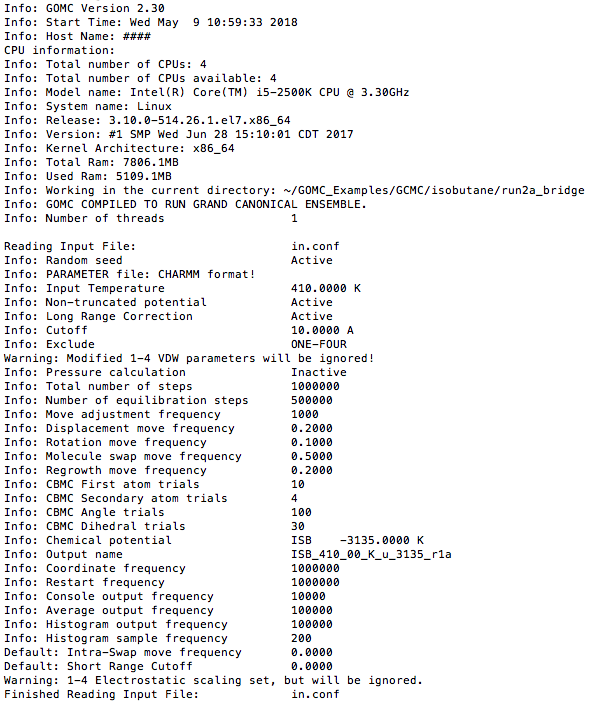
\includegraphics[scale=0.7]{images/out1}
\end{figure}
\begin{figure}[H]
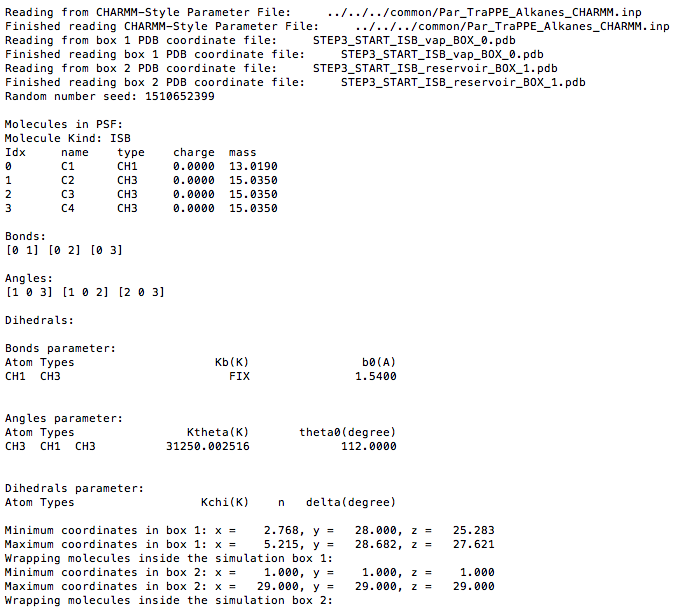
\includegraphics[scale=0.7]{images/out2}
\end{figure}
\newpage
Next, the energy and statistic title, initial energy and statistic of the system's starting configuration will print:\\
\colorbox{yellow}{\texttt{NOTE:}} If total energy of simulation is greater that $1.0 e^{14}$, \texttt{System Total Energy Calculation} will be performed at \texttt{EqSteps} to preserve energy value.
\begin{figure}[H]
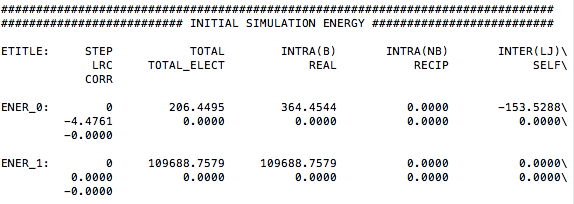
\includegraphics[scale=0.7]{images/out3}
\end{figure}
After the simulation starts, move, energy, and statistical title, followed by their values for each simulation box, will print:
\begin{figure}[H]
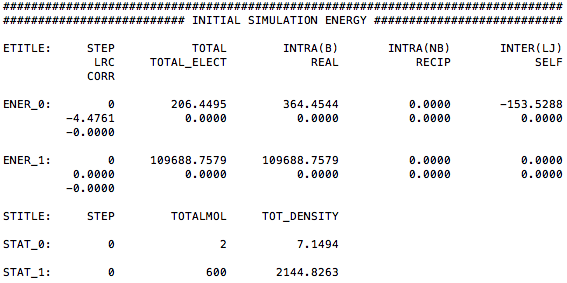
\includegraphics[scale=0.7]{images/out4}
\end{figure}
At the end of the run, timing information and other wrap up info will be printed.\\\\
\colorbox{yellow}{\texttt{NOTE:}} Printed energy and statistical values are instantaneous values.\\
\colorbox{yellow}{\texttt{NOTE:}} In order to keep the format of console file consistent, if absolute value of calculated properties of simulation is greater that $1.0 e^{11}$, the value of 999999999 will be printed instead.\\
\colorbox{yellow}{\texttt{NOTE:}} Since mol fraction value is very small compare to other properties, 8 digit precision was used instead of 4 digit to print out the value.\\
\colorbox{yellow}{\texttt{NOTE:}} It's important to watch the acceptance rates and adjust the move percentages and CBMC trial amounts to get the desired rate of move acceptance.

%Blockoutput section
\subsection{Block Output Files}
GOMC tracks a number of thermodynamic variables of interest during the simulation and prints them all in one file for each box.
\begin{itemize}
\item Energy
	\begin{itemize}
	\item Intermolecular (LJ)
	\item Intramolecular bonded
	\item Intramolecular nonbonded
	\item Tail corrections
	\item Electrostatic real
	\item Electrostatic Reciprocal
	\item Total Energy (sum of the all energies)
	\end{itemize}
\item Virial
\item Pressure 
\item Surface Tension (using virial method)
\item Volume
\item Total molecule number
\item Total Density
\item Mole fraction of each species
\item Heat of vaporization
\end{itemize}
At the beginning of each file, the title of each property followed by their average values is printed. Desired data can be extracted, as explained before, using the ``awk'' command. For example, in order to extract total density of the system, the following command need to be executed in terminal:\\\\
\colorbox{lightgray}{
\texttt{cat Blk\_OutputName\_BOX\_0.dat | awk `\{{print \$13}\}'}
}\\\\
Here, ``Blk\_OutputName\_BOX\_0.dat'' is the block-average file for simulation box 0 and ``\$13'' represents the 13th column of the block file.\\

\colorbox{yellow}{\texttt{NOTE:}} In order to keep the format of console file consistent, if absolute value of calculated properties of simulation is greater that $1.0 e^{11}$, the value of 999999999 will be printed instead.\\
\colorbox{yellow}{\texttt{NOTE:}} Since mol fraction value is very small compare to other properties, 8 digit precision was used instead of 4 digit to print out the value.\\

%Visualizing
\subsection{Visualizing Simulation}
If \texttt{CoordinatesFreq} is enabled in configuration file, GOMC will output the molecule coordinates every specified stpes.
The PDB and PSF output (merging of atom entries) has already been mentioned/explained in previous sections.  To recap: The PDB file's \texttt{ATOM} entries' occupancy is used to represent the box the molecule is in for the current frame. All molecules are listed in order in which they were read (i.e. if box 0 has 1..N1 molecules and box 1 has $1..N_2$ molecules, then all of the molecules in box 0 are listed first and all the molecules in box 1, i.e. $1..N_1, N_1+1..N_1+N_2$).  PDB frames are written as standard PDBs to consecutive file frames.\\\\
To visualize, open the output PDB and PSF files by GOMC using VMD,  type this command in the terminal:\\\\
For all simulation except Gibbs ensemble that has one simulation box:\\\\
\colorbox{lightgray}{
\texttt{\$ vmd ISB\_T\_270\_k\_merged.psf  ISB\_T\_270\_k\_BOX\_0.pdb}
}\\\\

For Gibbs ensemble, visualizing the first box:\\\\
\colorbox{lightgray}{
\texttt{\$ vmd ISB\_T\_270\_k\_merged.psf  ISB\_T\_270\_k\_BOX\_0.pdb}
}\\\\
For Gibbs ensemble, visualizing the second box:\\\\
\colorbox{lightgray}{
\texttt{\$ vmd ISB\_T\_270\_k\_merged.psf  ISB\_T\_270\_k\_BOX\_1.pdb}
}\\\\

\colorbox{yellow}{\texttt{NOTE:}} Restart coordinate file (OutputName\_BOX\_0\_restart.pdb) cannot be visualize using merged psf file, because atom number does not match. However, you can still open it in vmd using following command and vmd will automatically find the bonds of the molecule based on the coordinates.\\\\
\colorbox{lightgray}{
\texttt{\$ vmd  ISB\_T\_270\_k\_BOX\_0\_restart.pdb}
}\\\\

\newpage
%RUNNING
\section{Putting it all together: Running a GOMC Simulation}
It is strongly recommended that you download the test system provided at\\
\url{http://gomc.eng.wayne.edu/downloads.html} or \\
\url{https://github.com/GOMC-WSU/GOMC_Examples/tree/master}\\\\
Run different simulation types in order to become more familiar with different parameter and configuration files (*.conf).\\
To recap the previous examples, a simulation of isobutane will be completed for a single temperature point on the saturated vapor-liquid coexistence curve.\\
The general plan for running the simulation is:
\begin{enumerate}
\item Build GOMC (if not done already)
\item Copy GOMC executable to build directory
\item Create scripts, PDB, and topology file to build the system, plus in.dat file and parameter files to prepare for runtime
\item Build finished PDBs and PSFs using the simulation.
\item Run the simulation in the terminal.
\item Analyze the output.
\end{enumerate}
Please, complete steps 1 and 2; then, traverse to the directory, which should now contain a single file ``GOMC\_CPU\_GEMC''.
Next, six files need to be made:
\begin{itemize}
\item PDB file for isobutane
\item Topology file describing isobutane residue
\item Two *.inp packmol scripts to pack two system boxes
\item Two TCL scripts to input into PSFGen to generate the final configuration
\end{itemize}
\textbf{isobutane.pdb}\\

\colorbox{lightgray}{
\begin{tabular}{l *{8}{r}}
  \texttt{REMARK} & \texttt{1 File} & \texttt{created}  & \texttt{by} & \texttt{GaussView} & \texttt{5.0.8} & & & \\
  \texttt{ATOM} & \texttt{1} & \texttt{C1} & \texttt{ISB} & \texttt{1} & \texttt{0.911} & \texttt{-0.313} & \texttt{0.000}  & \texttt{C} \\
  \texttt{ATOM} & \texttt{2} & \texttt{C2} & \texttt{ISB} & \texttt{1} & \texttt{1.424} & \texttt{-1.765} & \texttt{0.000}  & \texttt{C} \\
  \texttt{ATOM} & \texttt{3} & \texttt{C3} & \texttt{ISB} & \texttt{1} & \texttt{-0.629} & \texttt{-0.313} & \texttt{0.000}  & \texttt{C} \\
  \texttt{ATOM} & \texttt{4} & \texttt{C4} & \texttt{ISB} & \texttt{1} & \texttt{1.424} & \texttt{0.413} & \texttt{-1.257} & \texttt{C} \\
  \multicolumn{9}{l}{\texttt{END}} \\
\end{tabular} 
} \\\\


\textbf{Top\_Branched\_Alkane.inp}\\
\colorbox{lightgray}{
\begin{tabular}{l}
\texttt{* Custom top file -- branched alkanes}\\
\texttt{*}\\
\texttt{MASS   1  CH3    15.035 C  !}\\
\texttt{MASS   2  CH1    13.019 C  !}\\\\
\texttt{AUTOGENERATE ANGLES DIHEDRALS}\\\\
\texttt{RESI ISB        0.00 ! isobutane – TraPPE}\\
\texttt{GROUP}\\
\texttt{ATOM C1 CH1     0.00 !      C3}\\
\texttt{ATOM C2 CH3     0.00 ! C2-C1}\\
\texttt{ATOM C3 CH3     0.00 !      C4}\\
\texttt{ATOM C4 CH3     0.00 !}\\
\texttt{BOND C1 C2 C1 C3 C1 C4}\\
\texttt{PATCHING FIRS NONE LAST NONE}\\
\texttt{END}\\
\end{tabular}}\\\\
\newline
\textbf{pack\_box\_0.inp}\\
\colorbox{lightgray}{
\begin{tabular}{l}
\texttt{tolerance 3.0}\\
\texttt{filetype pdb}\\
\texttt{output STEP2\_ISB\_packed\_BOX\_0.pdb}\\
\texttt{}\\
\texttt{structure isobutane.pdb}\\
\texttt{number 1000 }\\
\texttt{inside box 0. 0. 0. 68.00 68.00 68.00}\\
\texttt{end structure}\\
\end{tabular}}\\\\
\newline
\textbf{pack\_box\_1.inp}\\
\colorbox{lightgray}{
\begin{tabular}{l}
\texttt{tolerance 3.0}\\
\texttt{filetype pdb}\\
\texttt{output STEP2\_ISB\_packed\_BOX\_1.pdb}\\
\texttt{}\\
\texttt{structure isobutane.pdb}\\
\texttt{number 1000 }\\
\texttt{inside box 0. 0. 0. 68.00 68.00 68.00}\\
\texttt{end structure}\\
\end{tabular}}\\\\
\newline
\textbf{build\_box\_0.inp}\\
\colorbox{lightgray}{
\begin{tabular}{l}
\texttt{psfgen << ENDMOL}\\
\texttt{topology ./Top\_Branched\_Alkane.inp}\\
\texttt{segment ISB \{}\\
\texttt{    pdb ./STEP2\_ISB\_packed\_BOX\_0.pdb}\\
\texttt{    first none}\\
\texttt{    last none}\\
\texttt{\}}\\
\texttt{coordpdb ./STEP2\_ISB\_packed\_BOX\_0.pdb ISB}\\
\texttt{writepsf ./STEP3\_START\_ISB\_sys\_BOX\_0.psf}\\
\texttt{writepdb ./STEP3\_START\_ISB\_sys\_BOX\_0.pdb}\\
\end{tabular}}\\\\
\newline
\textbf{build\_box\_1.inp}\\
\colorbox{lightgray}{
\begin{tabular}{l}
\texttt{psfgen << ENDMOL}\\
\texttt{topology ./Top\_Branched\_Alkane.inp}\\
\texttt{segment ISB \{}\\
\texttt{    pdb ./STEP2\_ISB\_packed\_BOX\_1.pdb}\\
\texttt{    first none}\\
\texttt{    last none}\\
\texttt{\}}\\
\texttt{coordpdb ./STEP2\_ISB\_packed\_BOX\_1.pdb ISB}\\
\texttt{writepsf ./STEP3\_START\_ISB\_sys\_BOX\_1.psf}\\
\texttt{writepdb ./STEP3\_START\_ISB\_sys\_BOX\_1.pdb}\\
\end{tabular}}\\\\
These files can be created with a standard Linux or Windows text editor.  Please, also copy a Packmol executable into the working directory.\\\\
Once those files are created, run in the terminal:\\
\colorbox{lightgray}{
\begin{tabular}{l}
\texttt{./packmol < pack\_box\_0.inp}\\
\texttt{./packmol < pack\_box\_1.inp}\\
\end{tabular}}\\\\
This will create the intermediate PDBs.\\\\
Then, run the PSFGen scripts to finish the system using the following commands:\\
\colorbox{lightgray}{
\begin{tabular}{l}
\texttt{vmd < ./build\_box\_0.inp}\\
\texttt{vmd < ./build\_box\_1.inp}\\
\end{tabular}}\\\\
This will create the intermediate PDBs.\\
To run the code a few additional things will be needed:
\begin{itemize}
\item A GOMC Gibbs ensemble executable
\item A control file
\item Parameter files.
\end{itemize}
Enter the control file (in.conf) in the text editor in order to modify it. Example files for different simulation types can be found in previous section. \\
Once these four files have been added to the output directory, the simulation is ready.\\\\
Assuming the code is named \texttt{GOMC\_CPU\_GEMC}, run in the terminal using:\\
\colorbox{lightgray}{
\begin{tabular}{l}
\texttt{./GOMC\_CPU\_GEMC in.conf > out\_ISB\_T\_330.00\_K\_RUN\_0.log \&}
\end{tabular}}\\\\
For running GOMC in parallel, using openmp, run in the terminal using:\\
\colorbox{lightgray}{
\begin{tabular}{l}
\texttt{./GOMC\_CPU\_GEMC +p4 in.conf > out\_ISB\_T\_330.00\_K\_RUN\_0.log \&}
\end{tabular}}\\\\
Here, 4 defines the number of processors that will be used to run the simulation in parallel.\\\\
Progress can be monitored in the terminal with the tail command:\\
\colorbox{lightgray}{
\begin{tabular}{l}
\texttt{tail $-$f out\_ISB.log}
\end{tabular}}\\\\
\textcolor{green}{\texttt{Congratulations!}} You have examined a single-phase coexistence point on the saturated vapor-liquid curve using GOMC operating in the Gibbs ensemble.
\begin{figure}[H]
\centering
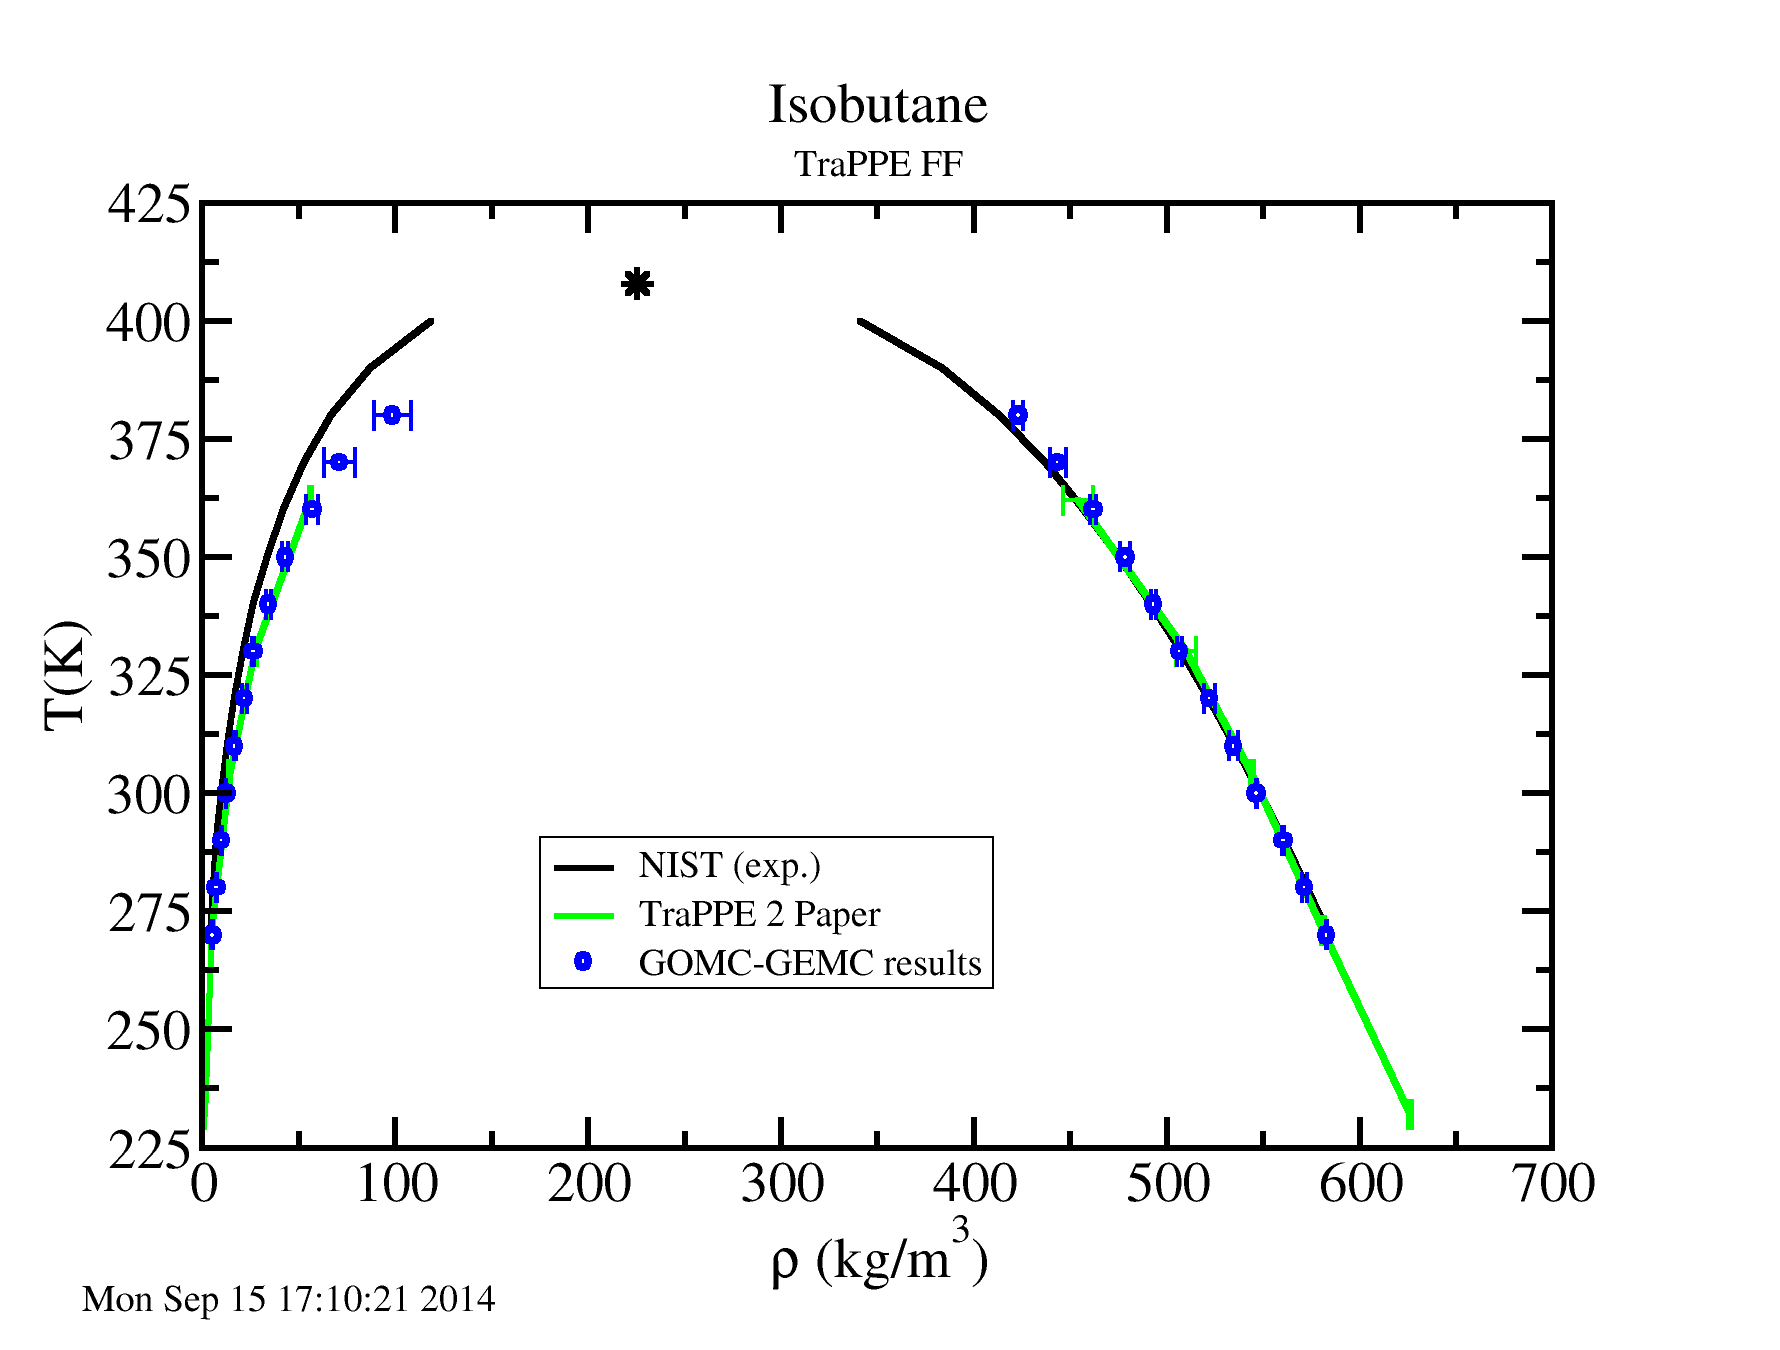
\includegraphics[scale=0.5]{images/isobutane_result}
\caption{Repeating this process for multiple temperatures will allow you to obtain the following results.}
\end{figure}
\newpage

%ntermolecular Energy
\section{Intermolecular Energy and Virial function (Van der Waals)}
In this section, the virial and energy equation of Van der Waals interaction for different potential function are discussed in details.
\subsection{VDW} This option calculates potential energy without any truncation.

\begin{itemize}
	\item Potential Calculation: Interactions between atoms can be modeled with an n$-$6 potential, a Mie potential in which the attractive exponent is fixed. The Mie potential can be viewed as a generalized version of the 12-6 Lennard-Jones potential, \\
\begin{equation}
E_{ij} = C_{n_{ij}} \epsilon_{ij} \bigg[\bigg(\frac{\sigma_{ij}}{r_{ij}}\bigg)^{n_{ij}} - \bigg(\frac{\sigma_{ij}}{r_{ij}}\bigg)^6\bigg]
\end{equation}

where $r_{ij}$, $\epsilon_{ij}$, and $\sigma_{ij}$ are, respectively, the separation, well depth, and collision diameter for the pair of interaction sites $i$ and $j$. The constant $C_n$ is a normalization factor such that the minimum of the potential remains at $-\epsilon_{ij}$ for all $n_{ij}$. In the 12-6 potential, $C_n$ reduces to the familiar value of 4.
\begin{equation}
C_{n_{ij}} = \bigg(\frac{n_{ij}}{n_{ij} - 6} \bigg)\bigg(\frac{n_{ij}}{6} \bigg)^{6/(n_{ij} - 6)}
\end{equation}

	\item Virial Calculation: Virial is basically the negative derivative of energy with respect to distance, multiplied by distance.\\
\begin{equation}
W_{ij} = -\frac{dE_{ij}}{dr}\times \frac{\rightharpoonup{r_{ij}}}{r_{ij}}
\end{equation}
Using n$-$6 LJ potential defined above:
\begin{equation}
W_{ij} = 6C_{n_{ij}} \epsilon_{ij} \bigg[\frac{n_{ij}}{6} \times \bigg(\frac{\sigma_{ij}}{r_{ij}}\bigg)^{n_{ij}} - \bigg(\frac{\sigma_{ij}}{r_{ij}}\bigg)^6\bigg]\times \frac{\overrightarrow{r_{ij}}}{{r_{ij}}^2}
\end{equation}
\colorbox{yellow}{\texttt{NOTE:}} This option only evaluates the energy up to specified \texttt{Rcut} distance. Tail correction to energy and pressure can be specified to account for infinite cutoff distance.
\end{itemize}

%SHIFT
\subsection{SHIFT} This option forces the potential energy to be zero at \texttt{Rcut} distance.
\begin{itemize}
	\item Potential Calculation: Interactions between atoms can be modeled with an n$-$6 potential,
	\begin{equation}
E_{ij}(\texttt{shift}) = C_{n_{ij}} \epsilon_{ij} \bigg[\bigg(\frac{\sigma_{ij}}{r_{ij}}\bigg)^{n_{ij}} - \bigg(\frac{\sigma_{ij}}{r_{ij}}\bigg)^6\bigg] - C_{n_{ij}} \epsilon_{ij} \bigg[\bigg(\frac{\sigma_{ij}}{r_{cut}}\bigg)^{n_{ij}} - \bigg(\frac{\sigma_{ij}}{r_{cut}}\bigg)^6\bigg]
\end{equation}

where $r_{ij}$, $\epsilon_{ij}$, and $\sigma_{ij}$ are, respectively, the separation, well depth, and collision diameter for the pair of interaction sites $i$ and $j$. The constant $C_n$ is a normalization factor according to Eq. 3, such that the minimum of the potential remains at $-\epsilon_{ij}$ for all $n_{ij}$. In the 12-6 potential, $C_n$ reduces to the familiar value of 4.
	\item Virial Calculation: Virial is basically the negative derivative of energy with respect to distance, multiplied by distance, Eq. 4.\\
Using \texttt{SHIFT} potential function defined above:
\begin{equation}
W_{ij}(\texttt{shift}) = 6C_{n_{ij}} \epsilon_{ij} \bigg[\frac{n_{ij}}{6} \times \bigg(\frac{\sigma_{ij}}{r_{ij}}\bigg)^{n_{ij}} - \bigg(\frac{\sigma_{ij}}{r_{ij}}\bigg)^6\bigg]\times \frac{\overrightarrow{r_{ij}}}{{r_{ij}}^2}
\end{equation}
\end{itemize}
\begin{figure}[H]
\centering
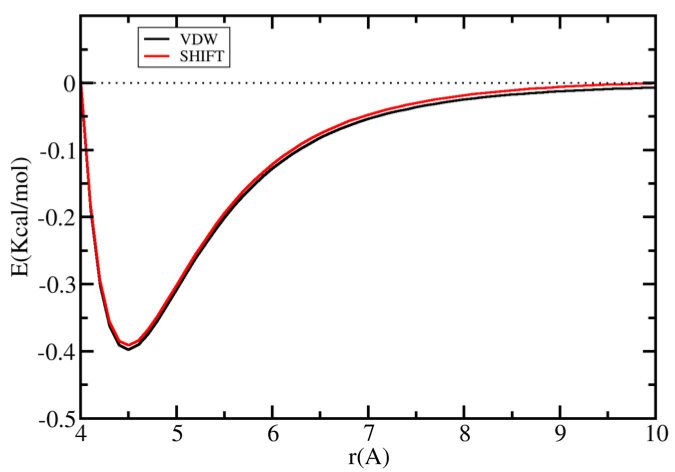
\includegraphics[scale=1.0]{images/VDW_SHIFT}
\caption{Graph of Van der Waals potential with and without the application of the \texttt{SHIFT} function. With the \texttt{SHIFT} function active, the potential by force was reduced to 0.0 at the \texttt{Rcut} distance. With the \texttt{SHIFT} function, there is a discontinuity where the potential is truncated.}
\end{figure}

%SWITCH 
\subsection{SWITCH} This option in \texttt{CHARMM} or \texttt{EXOTIC} force field smoothly forces the potential energy to be zero at \texttt{Rcut} distance and starts modifying the potential at \texttt{Rswitch} distance.
\begin{itemize}
	\item Potential Calculation: Interactions between atoms can be modeled with an n$-$6 potential,
	\begin{equation}
E_{ij}(\texttt{switch}) = C_{n_{ij}} \epsilon_{ij} \bigg[\bigg(\frac{\sigma_{ij}}{r_{ij}}\bigg)^{n_{ij}} - \bigg(\frac{\sigma_{ij}}{r_{ij}}\bigg)^6\bigg]\times F_E
	\end{equation}
	where $r_{ij}$, $\epsilon_{ij}$, and $\sigma_{ij}$ are, respectively, the separation, well depth, and collision diameter for the pair of interaction sites $i$ and $j$. The constant $C_n$ is a normalization factor according to Eq. 3, such that the minimum of the potential remains at $-\epsilon_{ij}$ for all $n_{ij}$. In the 12-6 potential, $C_n$ reduces to the familiar value of 4.\\\\
	The factor $F_E$ is defined as:
\[
	F_E = 
	\begin{cases}
		1 & r_{ij} \leq r_{switch} \\
		\frac{\big({r_{cut}}^2 - {r_{ij}}^2 \big)^2 \times \big({r_{cut}}^2 - 3{r_{switch}}^2 + 2{r_{ij}}^2 \big)}{\big({r_{cut}}^2 - {r_{switch}}^2 \big)^3} & r_{switch} < r_{ij} < r_{cut} \\
		0 & r_{ij} \geq r_{cut}
	\end{cases}
\]
\begin{equation}
\end{equation}
	
\item Virial Calculation: Virial is basically the negative derivative of energy with respect to distance, multiplied by distance, Eq. 4.\\
Using \texttt{SWITCH} potential function defined above:
\begin{equation}
W_{ij}(\texttt{switch}) = \Bigg[6 C_{n_{ij}} \epsilon_{ij} \bigg[\frac{n_{ij}}{6} \times \bigg(\frac{\sigma_{ij}}{r_{ij}}\bigg)^{n_{ij}} - \bigg(\frac{\sigma_{ij}}{r_{ij}}\bigg)^6\bigg]\times \frac{F_E}{{r_{ij}}^2}  - C_{n_{ij}} \epsilon_{ij} \bigg[\bigg(\frac{\sigma_{ij}}{r_{ij}}\bigg)^{n_{ij}} - \bigg(\frac{\sigma_{ij}}{r_{ij}}\bigg)^6\bigg] \times F_W \Bigg] \times \overrightarrow{r_{ij}}
\end{equation}
	The factor $F_W$ is defined as:
	\[
	F_W = 
	\begin{cases}
		1 & r_{ij} \leq r_{switch} \\
		\frac{12\big({r_{cut}}^2 - {r_{ij}}^2 \big) \times \big({r_{switch}}^2 - {r_{ij}}^2 \big)}{\big({r_{cut}}^2 - {r_{switch}}^2 \big)^3} & r_{switch} < r_{ij} < r_{cut} \\
		0 & r_{ij} \geq r_{cut}
	\end{cases}
\]
\begin{equation}
\end{equation}
\end{itemize}
\begin{figure}[H]
\centering
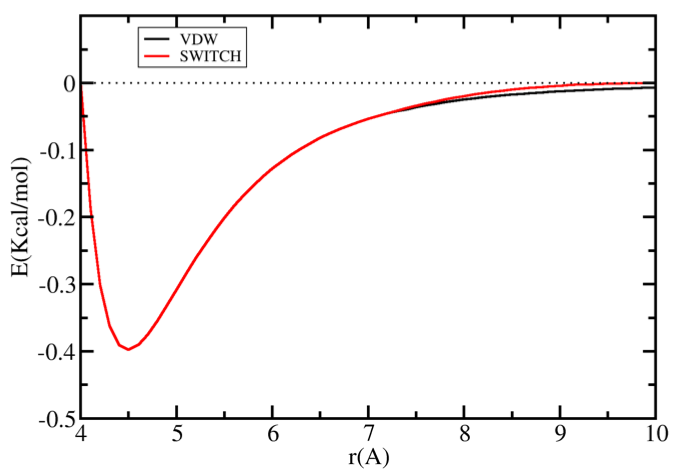
\includegraphics[scale=1.0]{images/SWITCH}
\caption{Graph of Van der Waals potential with and without the application of the \texttt{SWITCH }function. With the \texttt{SWITCH} function active, the potential is smoothly reduced to 0.0 at the \texttt{Rcut} distance. }
\end{figure}

%SWITCH MARTINI
\subsection{SWITCH (MARTINI)} This option in \texttt{MARTINI} force field smoothly forces the potential energy to be zero at \texttt{Rcut} distance and starts modifying the potential at \texttt{Rswitch} distance.
\begin{itemize}
	\item Potential Calculation: Interactions between atoms can be modeled with an n$-$6 potential. In standard \texttt{MARTINI}, $n$ is equal to 12,
	\begin{equation}
	E_{ij}(\texttt{switch}) = C_{n_{ij}}\epsilon_{ij} \Bigg[ {\sigma_{ij}}^{n} \bigg(\frac{1}{{r_{ij}}^{n}} + \varphi_{n} (r_{ij}) \bigg) - {\sigma_{ij}}^{6} \bigg(\frac{1}{{r_{ij}}^{6}} + \varphi_{6} (r_{ij}) \bigg) \Bigg]
	\end{equation}
where $r_{ij}$, $\epsilon_{ij}$, and $\sigma_{ij}$ are, respectively, the separation, well depth, and collision diameter for the pair of interaction sites $i$ and $j$. The constant $C_n$ is a normalization factor according to Eq. 3, such that the minimum of the potential remains at $-\epsilon_{ij}$ for all $n_{ij}$. In the 12-6 potential, $C_n$ reduces to the familiar value of 4.
\newpage
The factor $\varphi_{\alpha}$ and constants are defined as:

\[
	\varphi_{\alpha}(r_{ij}) = 
	\begin{cases}
		-C_{\alpha} & r_{ij} \leq r_{switch} \\
		-\frac{A_{\alpha}}{3} (r_{ij} - r_{switch})^3 -\frac{B_{\alpha}}{4} (r_{ij} - r_{switch})^4 - C_{\alpha} & r_{switch} < r_{ij} < r_{cut} \\
		0 & r_{ij} \geq r_{cut}
	\end{cases}
\]
\begin{equation}
\end{equation}
\begin{equation}
	A_{\alpha} = \alpha \frac{(\alpha + 1) r_{switch} - (\alpha +4) r_{cut}} {{r_{cut}}^{(\alpha + 2)} {(r_{cut} - r_{switch})}^2}
\end{equation}
\begin{equation}
	B_{\alpha} = \alpha \frac{(\alpha + 1) r_{switch} - (\alpha +3) r_{cut}} {{r_{cut}}^{(\alpha + 2)} {(r_{cut} - r_{switch})}^3}
\end{equation}
\begin{equation}
	C_{\alpha} =  \frac{1}{{r_{cut}}^{\alpha}} -\frac{A_{\alpha}}{3} (r_{cut} - r_{switch})^3 -\frac{B_{\alpha}}{4} (r_{cut} - r_{switch})^4
\end{equation}

\item Virial Calculation: Virial is basically the negative derivative of energy with respect to distance, multiplied by distance, Eq. 4.\\
Using the \texttt{SWITCH} potential function defined for \texttt{MARTINI} force field:

	\begin{equation}
	W_{ij}(\texttt{switch}) = C_{n_{ij}}\epsilon_{ij} \Bigg[ {\sigma_{ij}}^{n} \bigg(\frac{n}{{r_{ij}}^{(n+1)}} + d\varphi_{n} (r_{ij}) \bigg) - {\sigma_{ij}}^{6} \bigg(\frac{6}{{r_{ij}}^{(6+1)}} +d \varphi_{6} (r_{ij}) \bigg) \Bigg]\times \frac{\overrightarrow{r_{ij}}}{r_{ij}}
	\end{equation}
The constants defined in Eq. 14-16 and the factor $d\varphi_{\alpha}$ defined as:
\[
	d\varphi_{\alpha}(r_{ij}) = 
	\begin{cases}
		0 & r_{ij} \leq r_{switch} \\
		A_{\alpha} (r_{ij} - r_{switch})^2 + B_{\alpha} (r_{ij} - r_{switch})^3 & r_{switch} < r_{ij} < r_{cut} \\
		0 & r_{ij} \geq r_{cut}
	\end{cases}
\]
\begin{equation}
\end{equation}
\end{itemize}

\begin{figure}[H]
\centering
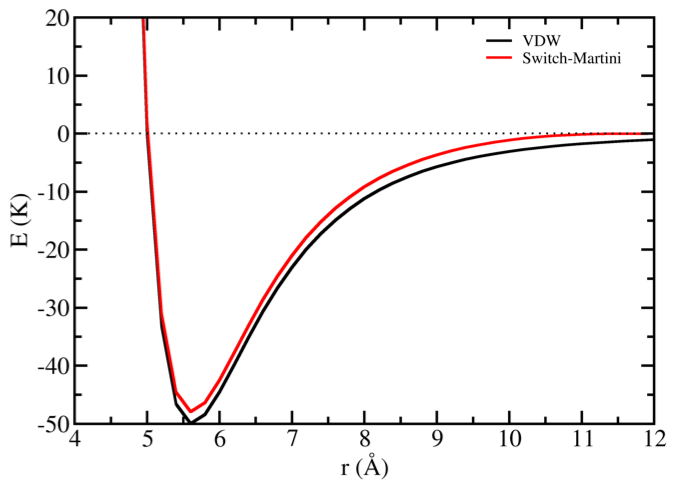
\includegraphics[scale=1.0]{images/MARTINI}
\caption{Graph of Van der Waals potential with and without the application of the \texttt{SWITCH} function in \texttt{MARTINI} force field. With the \texttt{SWITCH} function active, the potential is smoothly reduced to 0.0 at the \texttt{Rcut} distance.  }
\end{figure}	
\newpage

%Electrostatic
\section{Intermolecular Energy and Virial function (Electrostatic)}
In this section, the virial and energy equation of electrostatic interaction for different potential function are discussed in details.

\subsection{Ewald} This option calculate electrostatic energy using standard \texttt{Ewald Summation Method}. \\\\
\textit{\colorbox{yellow}{NOTE}: Once this option is activated, it would override the the electrostatic calculation using \texttt{VDW, SHIDT, and SWITCH} functions.}

\begin{itemize}
	\item Potential Calculation: Coulomb interactions between atoms can be modeled as
	\begin{equation}
		E(\texttt{Ewald}) = E_{real} + E_{reciprocal} + E_{self} + E_{correction}
	\end{equation}	
	$E_{real}$: Defines the short range electrostatic energy according to
	\begin{equation}
		E_{real} = \frac{1}{4\pi \epsilon_0} \frac{1}{2} \sum_{i =1}^{N} \sum_{j = 1}^{N} q_i q_j  \frac{\erfc(\alpha r_{ij})}{r_{ij}}
	\end{equation}
	, where $\alpha$ is \texttt{Ewald} separation parameter according to
	\begin{equation}
		\alpha = \frac {\sqrt{-\log (Tolerance)}}{r_{cut}}
	\end{equation}
	, where $Tolerance$ is a parameter, controlling the desired accuracy.\\

	$E_{reciprocal}$: Defines the long range electrostatic energy according to,
	\begin{equation}
		E_{reciprocal} = \frac{1}{\epsilon_0 V} \frac {1}{2} \sum_{\overrightarrow{k} \ne 0}^{} \frac {1}{\overrightarrow{k}^2}\exp\bigg(\frac {-\overrightarrow{k}^2}{4 \alpha^2}\bigg) \Bigg[ {\Big| R_{sum} \Big|}^2 + {\Big| I_{sum} \Big|}^2 \bigg]
	\end{equation}
	, where $\overrightarrow{k}$ is reciprocal vector, $R_{sum}$ and $I_{sum}$ are,
	\begin{equation}
	R_{sum} = \sum_{i=1}^{N} q_i \cos \big(\overrightarrow{k}.\overrightarrow{x_i}\big)
	\end{equation}
	\begin{equation}	
	I_{sum} = \sum_{i=1}^{N} q_i \sin \big(\overrightarrow{k}.\overrightarrow{x_i}\big)
	\end{equation}
	
	$E_{self}$: Defines the self energy according to,	
	\begin{equation}
	E_{self} = -\frac{\alpha}{4\pi \epsilon_0 \sqrt{\pi}} \sum_{i=1}^{N} {q_i}^2
	\end{equation}
	
	$E_{correction}$: Defines intra-molecule nonbonded enegy,	
	\begin{equation}
	E_{correction} = -\frac{1}{4\pi \epsilon_0} \frac{1}{2} \sum_{j=1}^{N }\sum_{l =1}^{N_j} \sum_{m = 1}^{N_j} q_{j_l} q_{j_m}  \frac{\erf(\alpha r_{j_l j_m})}{r_{j_l j_m}}
	\end{equation}

\item Virial Calculation: Virial is basically the negative derivative of energy with respect to distance, multiplied by distance, Eq. 4. Coulomb force between atoms can be modeled as,\\

	\begin{equation}
		W(\texttt{Ewald}) = W_{real} + W_{reciprocal} 
	\end{equation}
	
	$W_{real}$: Defines the short range electrostatic force according to,
	\begin{equation}
		W_{real} = \frac{1}{4\pi \epsilon_0} \frac{1}{2} \sum_{i =1}^{N} \sum_{j = 1}^{N} q_i q_j  \bigg[ \frac{\erfc(\alpha r_{ij})}{r_{ij}} + \frac{2\alpha}{ \sqrt{\pi}} \exp(-\alpha^2 {r_{ij}}^2) \bigg] \times \frac{\overrightarrow{r_{ij}}}{{r_{ij}}^2}
	\end{equation}
	
	$W_{reciprocal}$: Defines the long range electrostatic force according to,
	\begin{equation}
	\begin{split}
		W_{reciprocal} = \frac{1}{\epsilon_0 V} \frac {1}{2} \sum_{\overrightarrow{k} \ne 0}^{} \Bigg[\frac {1}{\overrightarrow{k}^2}\exp\bigg(\frac {-\overrightarrow{k}^2}{4 \alpha^2}\bigg) \bigg( {\Big| R_{sum} \Big|}^2 + {\Big| I_{sum} \Big|}^2 \bigg) \bigg(  1 - \frac{\overrightarrow{k}^2}{2\alpha^2} \bigg) \Bigg] +\\ 
\sum_{i=1}^{N} \frac{1}{\epsilon_0 V}  \sum_{\overrightarrow{k} \ne 0}^{} \Bigg[ \frac {q_i}{\overrightarrow{k}^2}\exp\bigg(\frac {-\overrightarrow{k}^2}{4 \alpha^2}\bigg) \bigg[ I_{sum} \times\cos(\overrightarrow{k}.\overrightarrow{x_i})  - R_{sum} \times \sin(\overrightarrow{k}.\overrightarrow{x_i}) \bigg] \Bigg] \times \big( \overrightarrow{k}.\overrightarrow{r_{ic}} \big)
	\end{split}
	\end{equation}
	, where $\overrightarrow{r_{ic}}$ is the vector between atom and the center of the mass of the molecule.
\end{itemize}

%SHIFT
\subsection{SHIFT} This option forces the electrostatic energy to be zero at \texttt{Rcut} distance.
\begin{itemize}
\item Potential Calculation: Coulomb interactions between atoms can be modeled as
	\begin{equation}
		E(\texttt{SHIFT}) = \frac{q_i q_j}{4\pi \epsilon_0} \Big( \frac{1}{r_{ij}} - \frac{1}{r_{cut}} \Big)
	\end{equation}	
\item Virial Calculation: Virial is basically the negative derivative of energy with respect to distance, multiplied by distance, Eq. 4. Coulomb force between atoms can be modeled as,\\
	\begin{equation}
		W(\texttt{SHIFT}) = \frac{q_i q_j}{4\pi \epsilon_0} \Big( \frac{1}{r_{ij}} \times \frac{\overrightarrow{r_{ij}}}{{r_{ij}}^2} \Big)
	\end{equation}	
\end{itemize}

%SWITCH
\subsection{SWITCH} This option in \texttt{CHARMM} or \texttt{EXOTIC} force field forces the electrostatic energy to be zero at \texttt{Rcut} distance.
\begin{itemize}
	\item Potential Calculation: Coulomb interactions between atoms can be modeled as,
	\begin{equation}
		E(\texttt{SWITCH}) = \frac{q_i q_j}{4\pi \epsilon_0} \bigg( \Big(\frac{r_{ij}}{r_{cut}} \Big)^2 - 1.0\bigg)^2 \frac{1}{r_{ij}}
	\end{equation}
	
	\item Virial Calculation: Virial is basically the negative derivative of energy with respect to distance, multiplied by distance, Eq. 4. Coulomb force between atoms can be modeled as,\\
	\begin{equation}
		W(\texttt{SWITCH}) = \frac{q_i q_j}{4\pi \epsilon_0} \Bigg[ \bigg( \Big(\frac{r_{ij}}{r_{cut}} \Big)^2 - 1.0\bigg)^2 \frac{1}{{r_{ij}}^2} - \bigg( \frac{4}{{r_{cut}}^2} \bigg) \bigg( \Big(\frac{r_{ij}}{r_{cut}} \Big)^2 - 1.0\bigg) \Bigg] \times \frac{\overrightarrow{r_{ij}}}{r_{ij}}
	\end{equation}	
\end{itemize}

%MARTINI
\subsection{SWITCH (MARTINI)} This option in \texttt{MARTINI} force field smoothly forces the potential energy to be zero at \texttt{Rcut} distance and starts modifying the potential at \texttt{"Rswitch = 0.0"} distance.
\begin{itemize}
	\item Potential Calculation: Coulomb interactions between atoms can be modeled as,
	\begin{equation}
		E(\texttt{SWITCH}) = \frac{q_i q_j}{4\pi \epsilon_0 \epsilon_1} \bigg( \frac{1}{r_{ij}} + \varphi_{1} (r_{ij}) \bigg)
	\end{equation}
	, where $\epsilon_1$ is the dielectric constant, which in \texttt{MARTINI} force field is equal to 15.0 and $\varphi_{\alpha} (r_{ij})$ is defined in Eq. 13-16.
	
	\item Virial Calculation: Virial is basically the negative derivative of energy with respect to distance, multiplied by distance, Eq. 4. Coulomb force between atoms can be modeled as,\\
	\begin{equation}
		W(\texttt{SWITCH}) =  \frac{q_i q_j}{4\pi \epsilon_0 \epsilon_1} \bigg( \frac{1}{{r_{ij}}^2} + d\varphi_1 (r_{ij})  \bigg) \times \frac{\overrightarrow{r_{ij}}}{r_{ij}}
	\end{equation}
	, where $d\varphi_1 (r_{ij})$ is defined in Eq. 18.	
\end{itemize}
\newpage

%Contact
\section{Get Help or Technical Support }

For get any help or technical support, please send message to \texttt{GOMC gitter}:\\\\
\url{https://gitter.im/GOMC_WSU/Lobby} \\\\
or send email to:\\
\begin{itemize}

	\item Jeffrey Potoff:  \texttt{jpotoff@wayne.edu}
	\item Loren Schwiebert: \texttt{loren@wayne.edu}
	
\end{itemize}


\end{document}